\documentclass[10pt,twocolumn]{article}
\usepackage[margin=0.75in]{geometry}
\usepackage{graphicx}
\usepackage{booktabs}
\usepackage{amsmath}
\usepackage{hyperref}
\usepackage{float}
\usepackage{caption}
\usepackage[numbers]{natbib}
\usepackage{enumitem}

\setlength{\columnsep}{0.25in}
\captionsetup{font=small, labelfont=bf}

\title{\textbf{Supervised Learning Report: Evaluating Four Algorithm Families on Adult Income and Wine Quality Datasets}}
\author{Max Montes Soza \\ CS7641 Machine Learning, Spring 2026}
\date{}

\begin{document}
\maketitle

% ============================================================
\section{Introduction}
% ============================================================

This report evaluates four supervised learning algorithm families (Decision Trees, k-Nearest Neighbors, Support Vector Machines, and Neural Networks) on two classification tasks: predicting income level from census data (Adult Income, binary) and predicting wine quality from physicochemical measurements (Wine Quality, multiclass). For each algorithm and dataset pair, we present learning curves, model-complexity curves, confusion matrices, and runtime profiling. All experiments use a single held-out test split evaluated once at the end; hyperparameter tuning is performed exclusively via cross-validation on the training set to prevent data leakage.

\subsection{Hypotheses}

\textbf{Adult Income.} We hypothesize that SVM (RBF) and neural networks will outperform DT and kNN. After one-hot encoding the eight categorical features, the original 14 features expand to 104 columns, mostly sparse binary indicators plus six continuous features. This high-dimensional space favors margin-based classifiers that can find optimal separating hyperplanes, while kNN should suffer from the curse of dimensionality as distances become less discriminative. The 3:1 class imbalance further advantages models with smooth, flexible boundaries that can better capture minority-class structure. \textit{Predicted ordering:} SVM (RBF) $\geq$ NN $>$ DT $>$ kNN.

\textbf{Wine Quality.} We hypothesize that DT and NN will perform best. All 13 features are continuous with no missing values, and the ordinal nature of quality ratings means adjacent classes overlap substantially. DTs handle multiclass problems naturally via recursive partitioning, while NNs with sufficient capacity can learn non-linear interactions between chemical properties. SVM may struggle with the multiclass decomposition and overlapping boundaries, while kNN should perform reasonably in the low-dimensional, continuous space. \textit{Predicted ordering:} NN $\geq$ DT $>$ kNN $>$ SVM.

% ============================================================
\section{Data, Targets, and Methodology}
% ============================================================

\textbf{Adult Income} contains 45{,}222 samples with 14 features (6 continuous, 8 categorical). The binary target is income ($\leq$50K vs.\ $>$50K) with a 3.03:1 class imbalance (34{,}014 vs.\ 11{,}208). No missing values are present. We evaluate with F1 score (primary) and accuracy, using F1 because accuracy alone is misleading under imbalance. A model predicting only the majority class achieves 75.2\% accuracy but F1$=$0.

\textbf{Wine Quality} contains 6{,}497 samples with 13 features (12 physicochemical measurements plus a red/white type indicator). The target is quality rating with eight classes (1--8), heavily imbalanced: classes 3--5 constitute 81.2\% of samples while classes 1, 2, 7, and 8 together account for only 6.2\%. We evaluate with Macro-F1 (primary) and accuracy, using Macro-F1 because it weights all classes equally regardless of frequency, ensuring rare quality levels receive equal consideration.

\textbf{Preprocessing.} For Adult, categorical features are one-hot encoded and numeric features are standardized via \texttt{StandardScaler}, producing a 104-dimensional feature vector. For Wine, all features are standardized. Preprocessing is fit on the training set only to prevent leakage. Features are split 80/20 (stratified, seed$=$42), yielding 36{,}177 training and 9{,}045 test samples for Adult, and 5{,}197 training and 1{,}300 test samples for Wine.

\textbf{Tuning.} DT and kNN use stratified 5-fold CV with \texttt{RandomizedSearchCV}. SVM and NN use Optuna (Bayesian optimization with TPE) with 3-fold stratified CV to reduce runtime. All models are evaluated on the same held-out test set for fair comparison.

\textbf{Leakage Controls.} All preprocessing transformations are fit within cross-validation folds or on the training split only. We verify evaluation integrity with a dummy baseline (most-frequent class) and a shuffled-label baseline, both detailed in Section~\ref{sec:leakage}.

% ============================================================
\section{Decision Trees}
% ============================================================

We train \texttt{DecisionTreeClassifier} with Gini impurity, tuning \texttt{max\_depth} $\in \{3, 5, 8, 10, 14, 18, \text{None}\}$, \texttt{min\_samples\_split} $\in \{2, 5, 10, 50, 100\}$, \texttt{min\_samples\_leaf} $\in \{1, 5, 10, 50, 100, 200\}$, and \texttt{ccp\_alpha} $\in \{0, 10^{-4}, 5\!\times\!10^{-4}, 10^{-3}, 5\!\times\!10^{-3}\}$ via RandomizedSearchCV (60 iterations). Gini is computationally efficient and performs comparably to entropy in practice~\cite{hastie2009elements}.

\textbf{Adult.} The best configuration uses \texttt{max\_depth}$=$18, \texttt{min\_samples\_split}$=$5, \texttt{ccp\_alpha}$=$0.0001, producing a tree with 128 leaves. The model achieves accuracy$=$0.854 and F1$=$0.670 with a fit time of 0.162s. The learning curve (Figure~\ref{fig:dt_adult}) shows a narrowing gap between training and validation scores as training size increases, indicating that pruning successfully controls overfitting. The model-complexity curve against \texttt{ccp\_alpha} shows that aggressive pruning ($\alpha > 0.005$) rapidly degrades performance, while the optimal region lies near $\alpha = 10^{-4}$. Feature importance analysis reveals that \texttt{marital-status}, \texttt{education-num}, and \texttt{capital-gain} are the strongest predictors.

\textbf{Wine.} The best DT uses \texttt{max\_depth}$=$14, \texttt{min\_samples\_split}$=$2, and \texttt{ccp\_alpha}$=$0, producing a larger tree with 942 leaves. It achieves accuracy$=$0.609 and Macro-F1$=$0.432. The unpruned tree reflects the difficulty of the multiclass problem: the model needs substantial depth to separate overlapping quality classes. The confusion matrix shows that the model concentrates predictions on majority classes (3--5) and struggles with rare classes (1, 2, 7, 8), a pattern consistent across all algorithms on this dataset.

\begin{figure}[H]
\centering
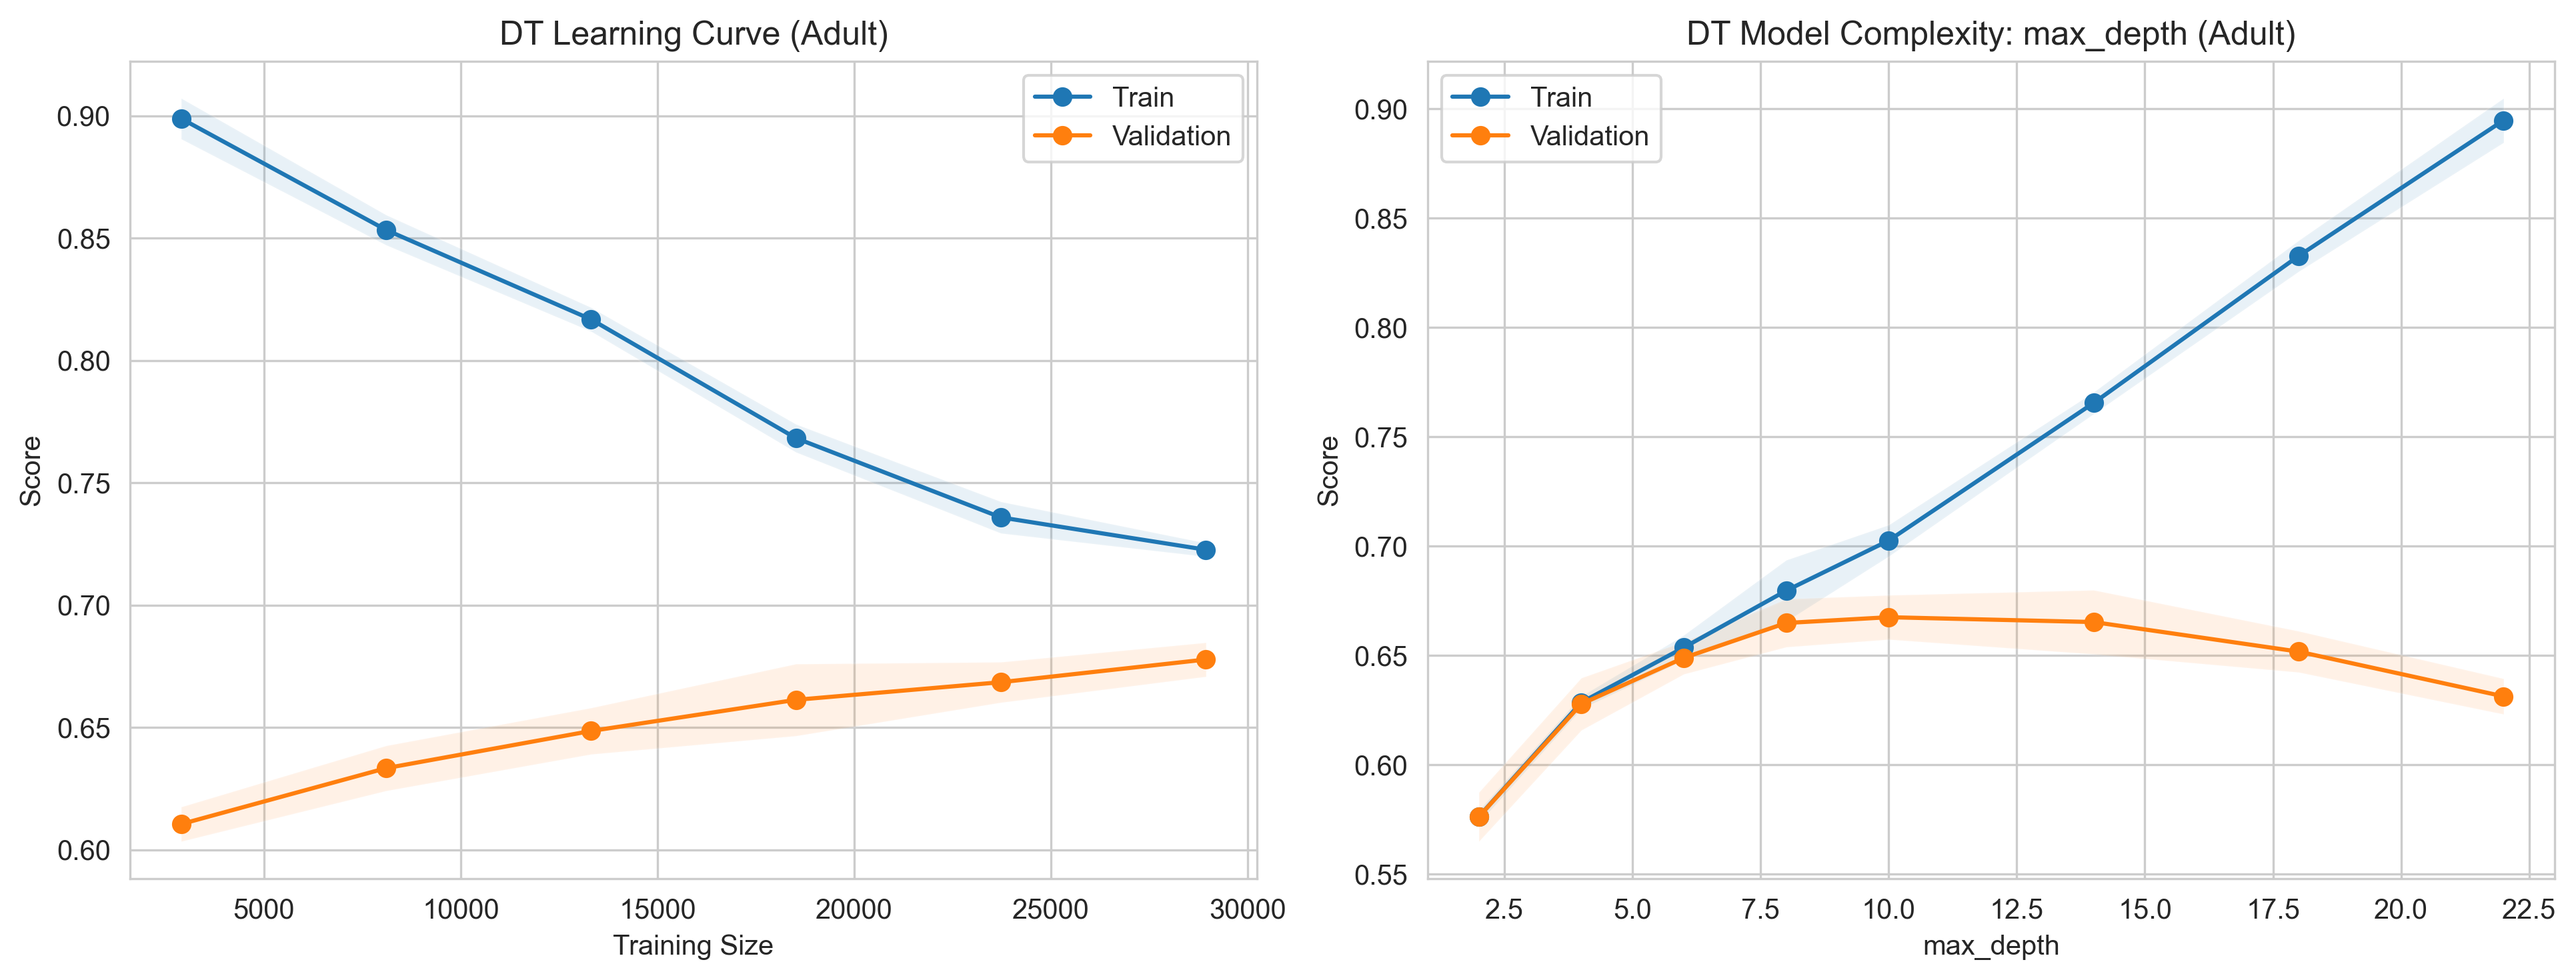
\includegraphics[width=\linewidth]{figures/dt_adult_curves.png}
\caption{DT learning curve and model-complexity curve (Adult). The LC shows convergent train/val scores with moderate pruning. The MC curve confirms $\text{ccp\_alpha} \approx 10^{-4}$ balances bias and variance.}
\label{fig:dt_adult}
\end{figure}

\begin{figure}[H]
\centering
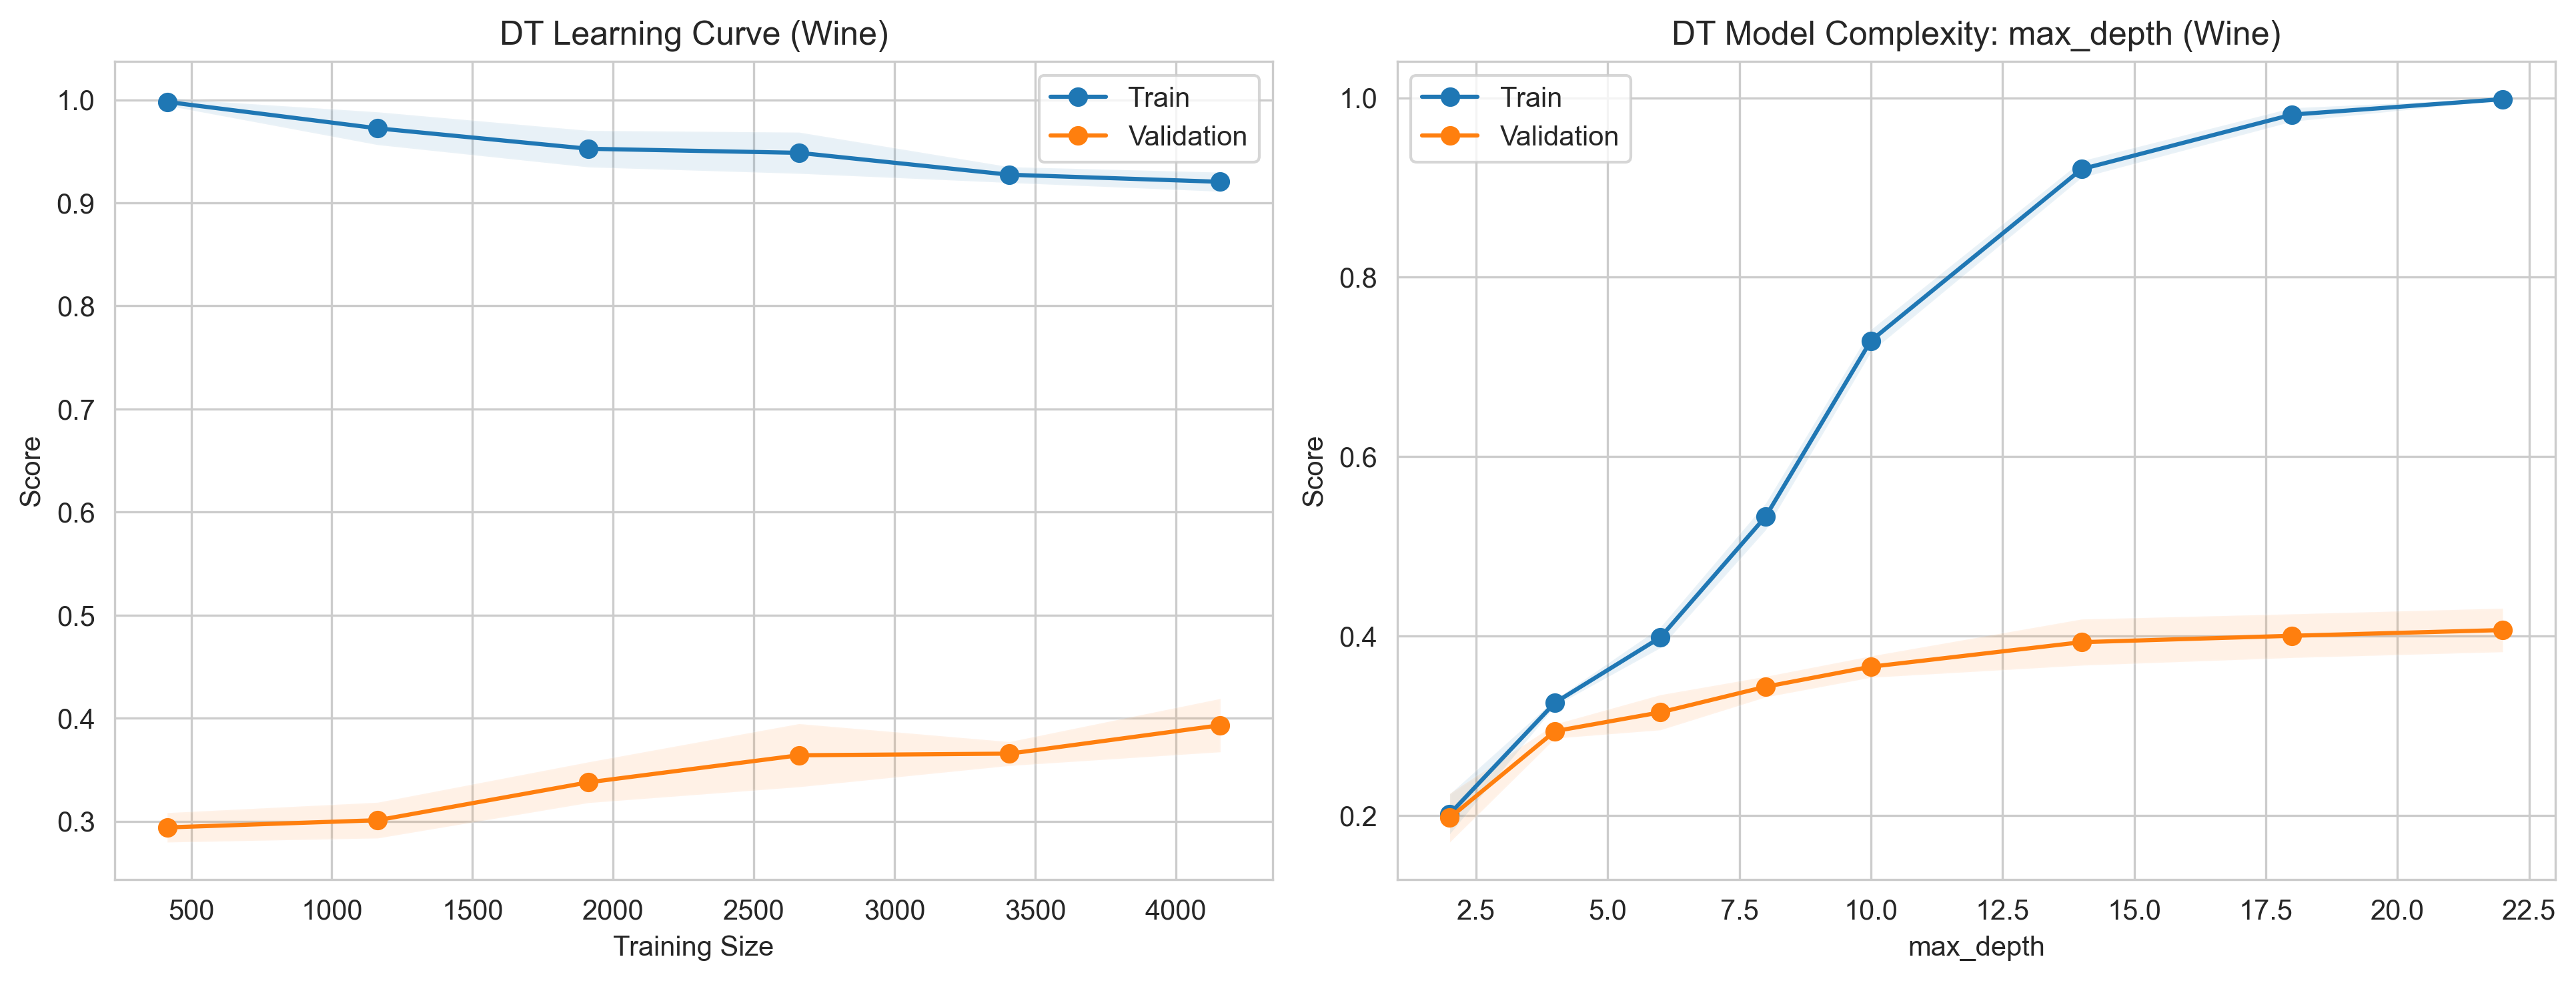
\includegraphics[width=\linewidth]{figures/dt_wine_curves.png}
\caption{DT learning curve and model-complexity curve (Wine). The persistent train--val gap signals high variance, consistent with the small dataset and many overlapping classes.}
\label{fig:dt_wine}
\end{figure}

% ============================================================
\section{k-Nearest Neighbors}
% ============================================================

We tune $k \in \{3, 5, 11, 21, 31, 51\}$, distance metric (Euclidean, Manhattan), and weighting scheme (uniform, distance) via \texttt{RandomizedSearchCV}. Features are standardized for all kNN experiments, as distance-based methods are sensitive to feature scales.

\textbf{Adult.} The best configuration is $k=21$, uniform weighting, Euclidean distance, achieving accuracy$=$0.836 and F1$=$0.642 with near-instantaneous fit (0.001s) but slow prediction (0.796s). The learning curve shows training F1 around 0.68 and validation F1 around 0.64, a relatively narrow gap that suggests the model has limited capacity to improve regardless of training size. The model-complexity curve against $k$ shows that smaller $k$ values overfit (high train, low val) while larger $k$ values smooth the boundary but plateau quickly. The large $k=21$ reflects the high-dimensional one-hot encoded space (104 features): with many irrelevant binary dimensions, more neighbors are needed to form a stable vote, confirming the curse-of-dimensionality hypothesis.

\textbf{Wine.} The best configuration is $k=11$, distance weighting, Manhattan distance, achieving accuracy$=$0.679 and Macro-F1$=$0.455. This is notably strong, placing second overall on Wine. The learning curve shows training F1 near 1.0 (expected for kNN, as each point is its own nearest neighbor in a small dataset) and validation F1 still climbing at maximum training size, suggesting more data would further improve performance. The selection of Manhattan distance over Euclidean is sensible for this dataset: Manhattan is more robust to outliers in individual chemical measurements. The low dimensionality (13 features) explains why kNN succeeds here but struggles on Adult. In 13 continuous dimensions, distances remain meaningful, and the local neighborhood structure captures real patterns. This contrast between datasets illustrates the no-free-lunch theorem: kNN's simplicity is a liability in high-dimensional sparse spaces but a strength in low-dimensional continuous ones.

\begin{figure}[H]
\centering
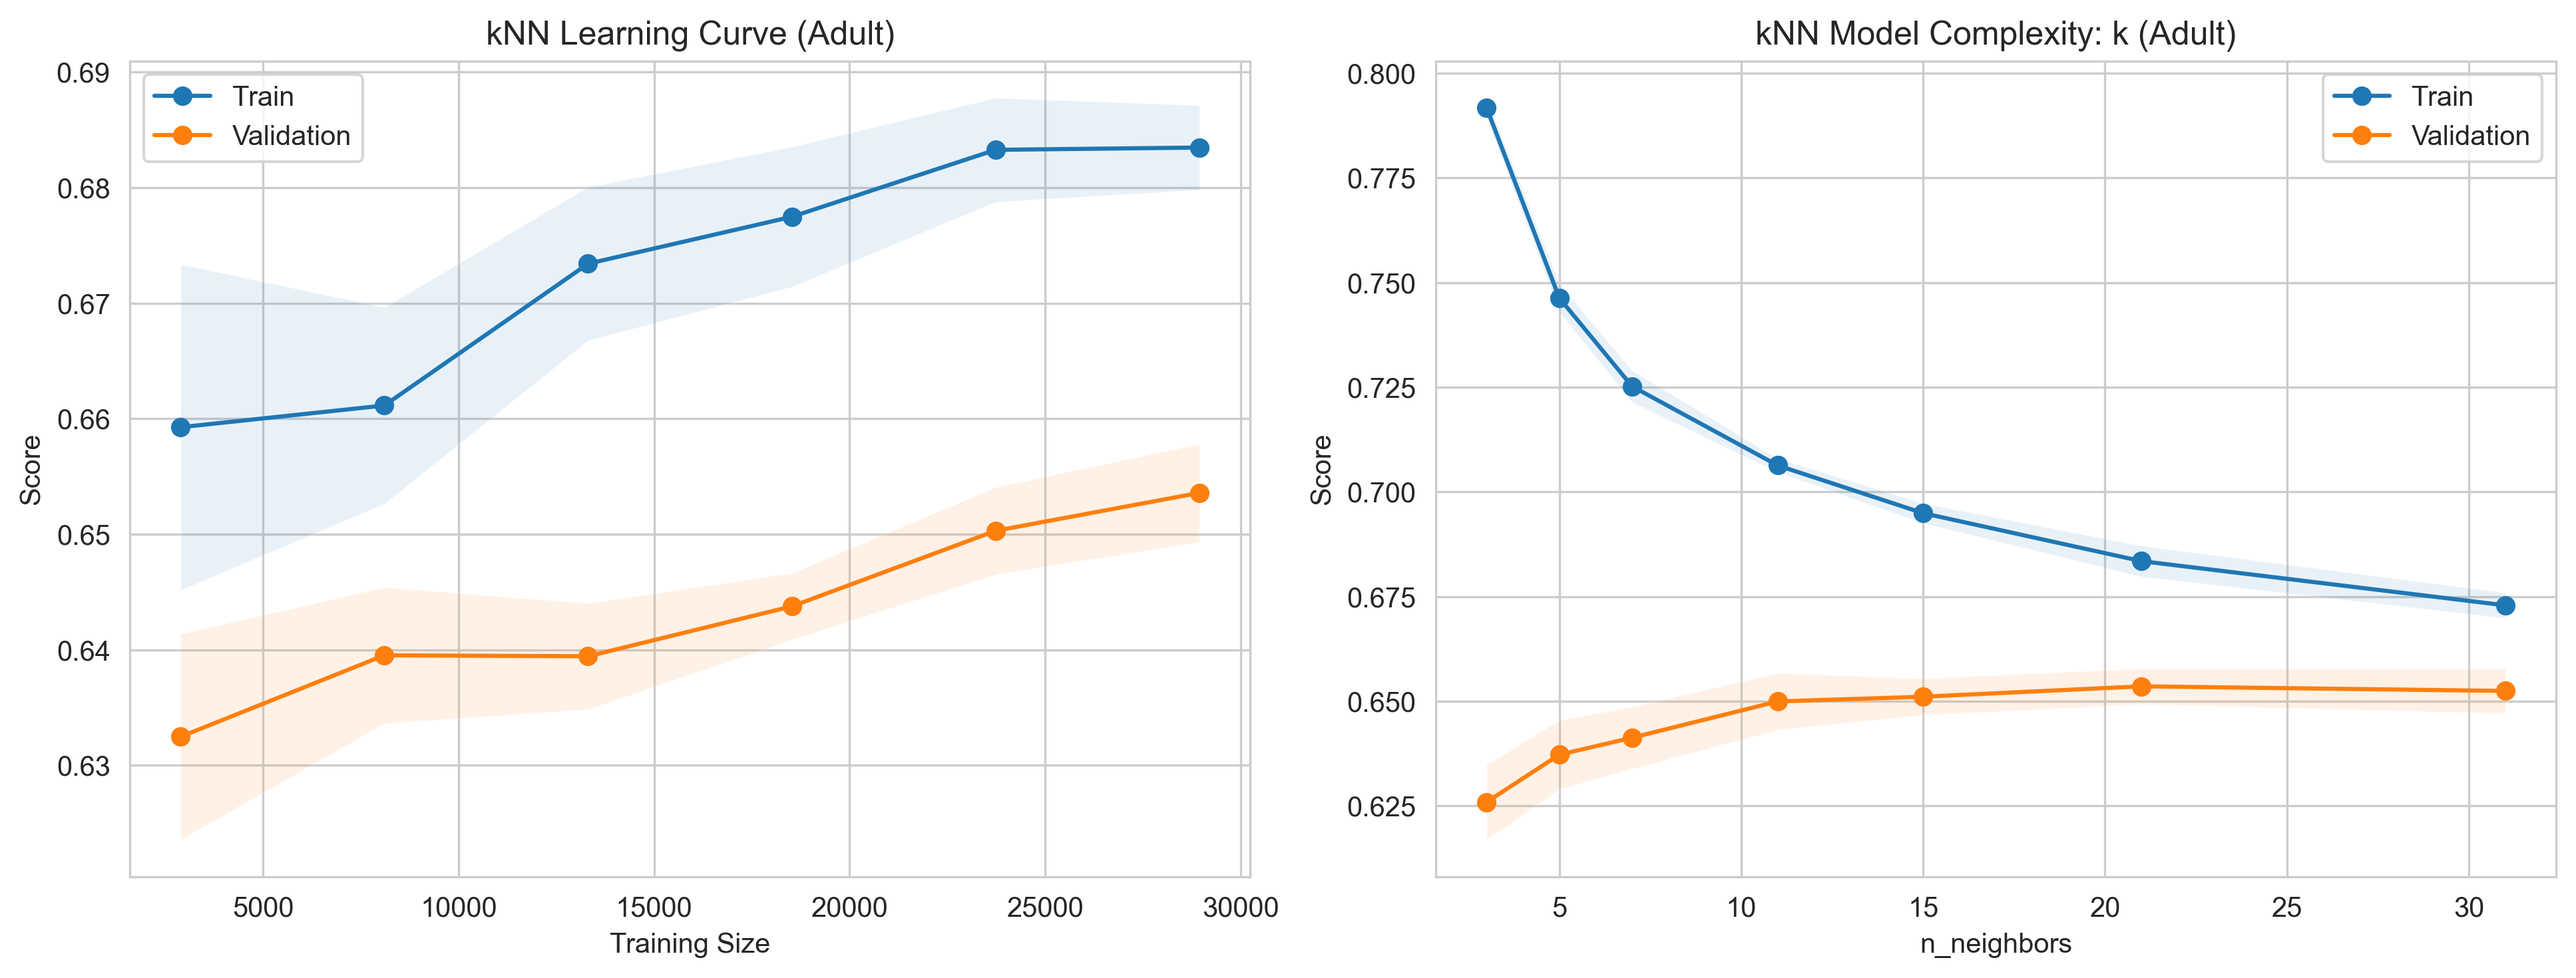
\includegraphics[width=\linewidth]{figures/knn_adult_curves.png}
\caption{kNN learning and model-complexity curves (Adult). The MC curve shows diminishing returns beyond $k=11$, and the LC indicates limited capacity in the high-dimensional space.}
\label{fig:knn_adult}
\end{figure}

\begin{figure}[H]
\centering
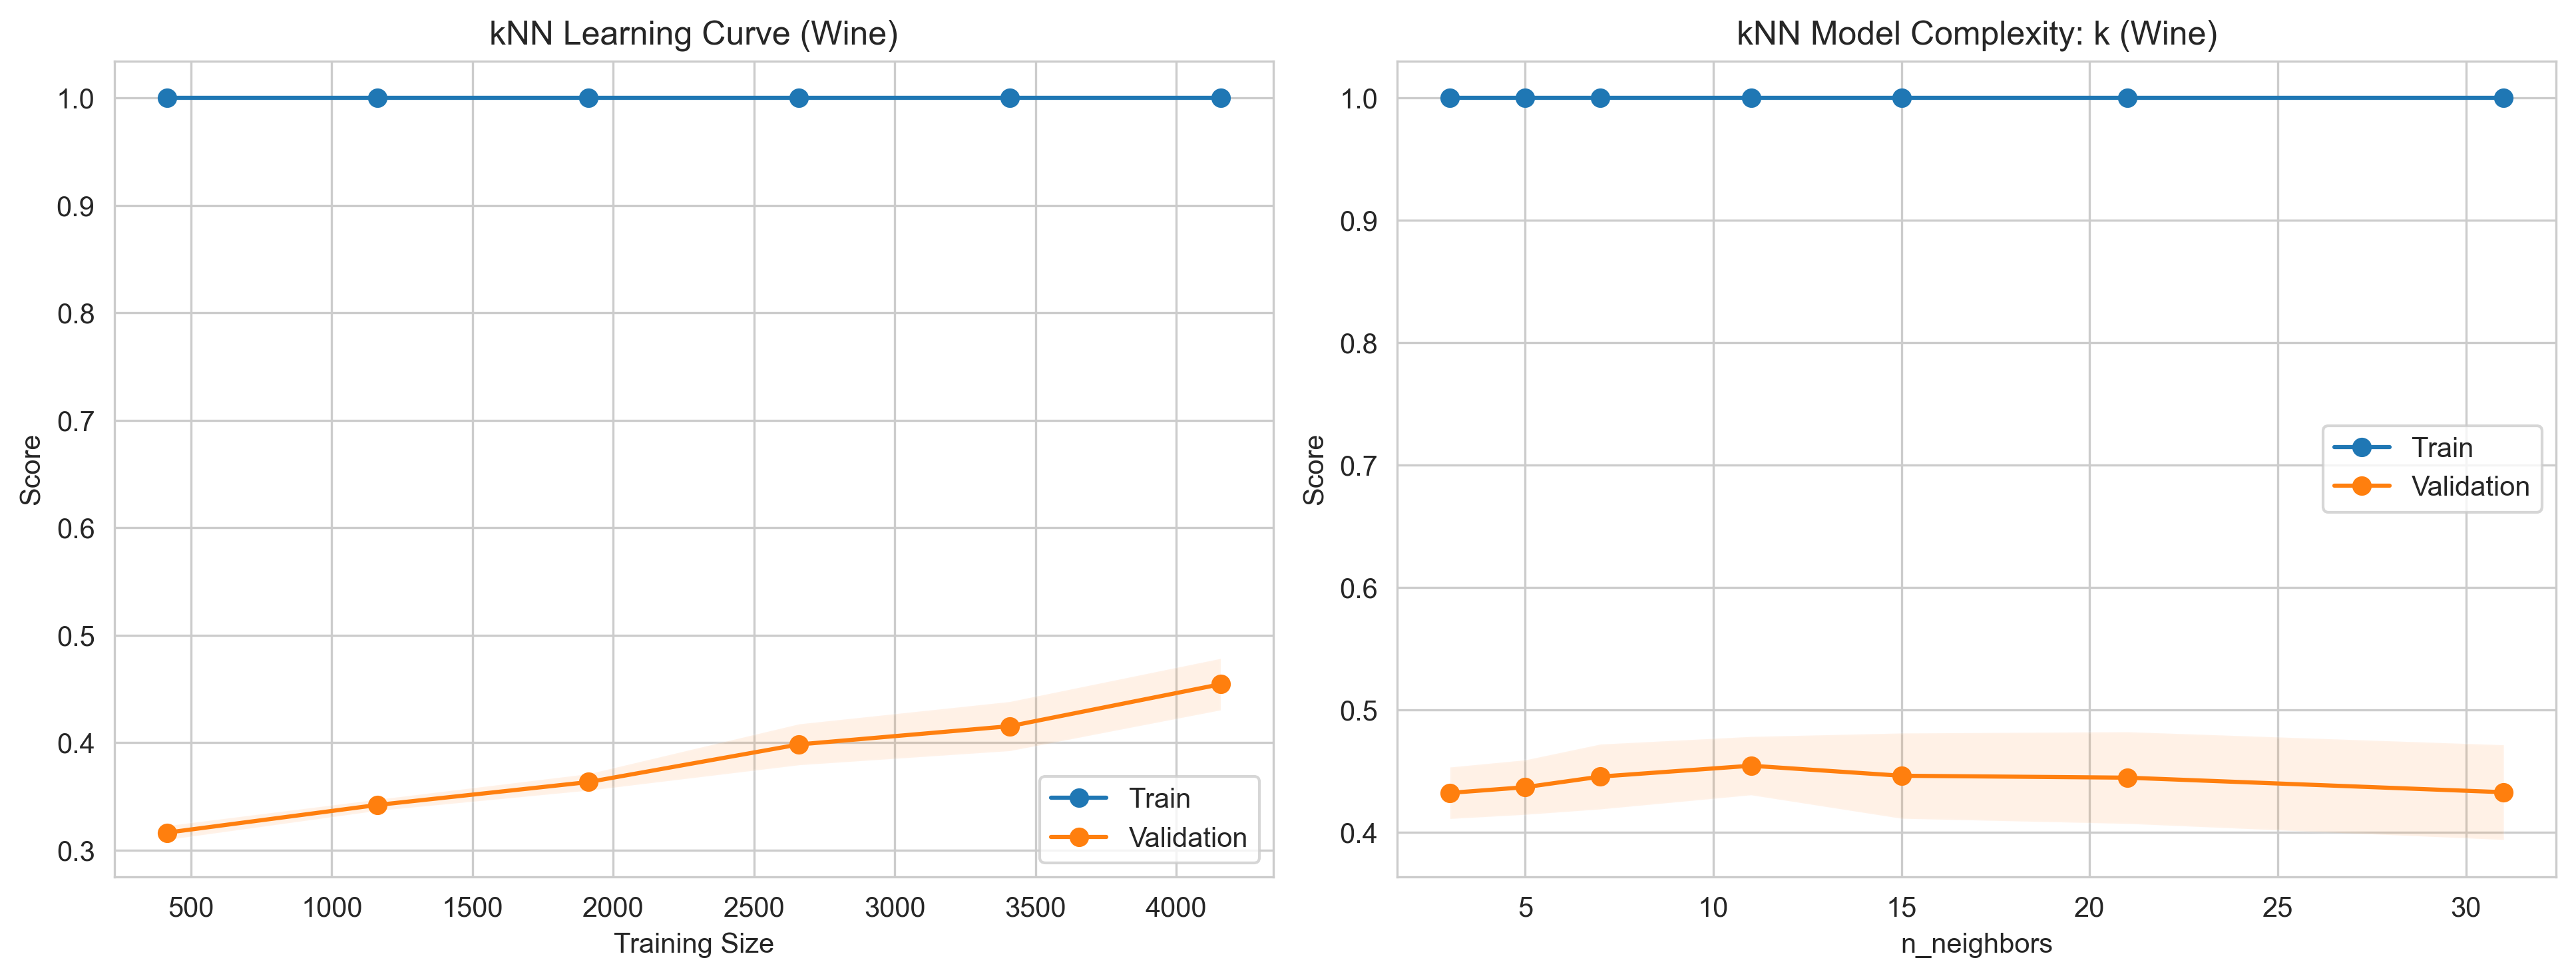
\includegraphics[width=\linewidth]{figures/knn_wine_curves.png}
\caption{kNN learning and model-complexity curves (Wine). The training F1 near 1.0 is a characteristic of kNN on small datasets (self-neighbor effect). The validation curve still rising at maximum training size suggests more data would help.}
\label{fig:knn_wine}
\end{figure}

% ============================================================
\section{Support Vector Machines}
% ============================================================

We evaluate two kernels per dataset (Linear and RBF) as required, tuning $C$ for both and $\gamma$ for RBF via Optuna. All features are standardized, which is essential for SVM since the margin-based objective is sensitive to feature scales. For the Adult dataset, the RBF SVM is trained on a 10{,}000-sample subsample due to the $O(n^2)$--$O(n^3)$ complexity of kernel SVMs; timing evidence justifies this decision (full training would require $>$30 minutes).

\textbf{Adult.} Linear SVM with $C=2.89$ achieves accuracy$=$0.846 and F1$=$0.654 (fit: 0.114s). RBF SVM with $C=11.50$ and $\gamma=0.023$ achieves accuracy$=$0.848 and F1$=$0.650 on the subsample (fit: 1.353s, predict: 2.393s). The nearly identical performance between kernels suggests the decision boundary is approximately linear in the high-dimensional one-hot encoded space, consistent with the Cover theorem: data projected into sufficiently high dimensions tends to become linearly separable. The model-complexity curve against $C$ for Linear SVM shows validation F1 rising sharply from $C=0.001$ to $C=1$, then plateauing, which indicates that the margin-misclassification tradeoff is satisfied at moderate regularization.

\textbf{Wine.} Linear SVM with $C=20.48$ achieves accuracy$=$0.518 and Macro-F1$=$0.253 (fit: 0.027s), while RBF SVM with $C=89.46$ and $\gamma=0.549$ substantially improves to accuracy$=$0.662 and Macro-F1$=$0.467 (fit: 0.480s, predict: 0.145s). The large performance gap between kernels reveals that the Wine quality boundaries are highly non-linear, which makes sense given the complex chemical interactions that determine quality. The high $\gamma$ value indicates tight decision boundaries that closely follow the training data, while the high $C$ penalizes misclassifications aggressively. Despite this, RBF SVM achieves the best single-model Macro-F1 on Wine, outperforming models with far more parameters.

\begin{figure}[H]
\centering
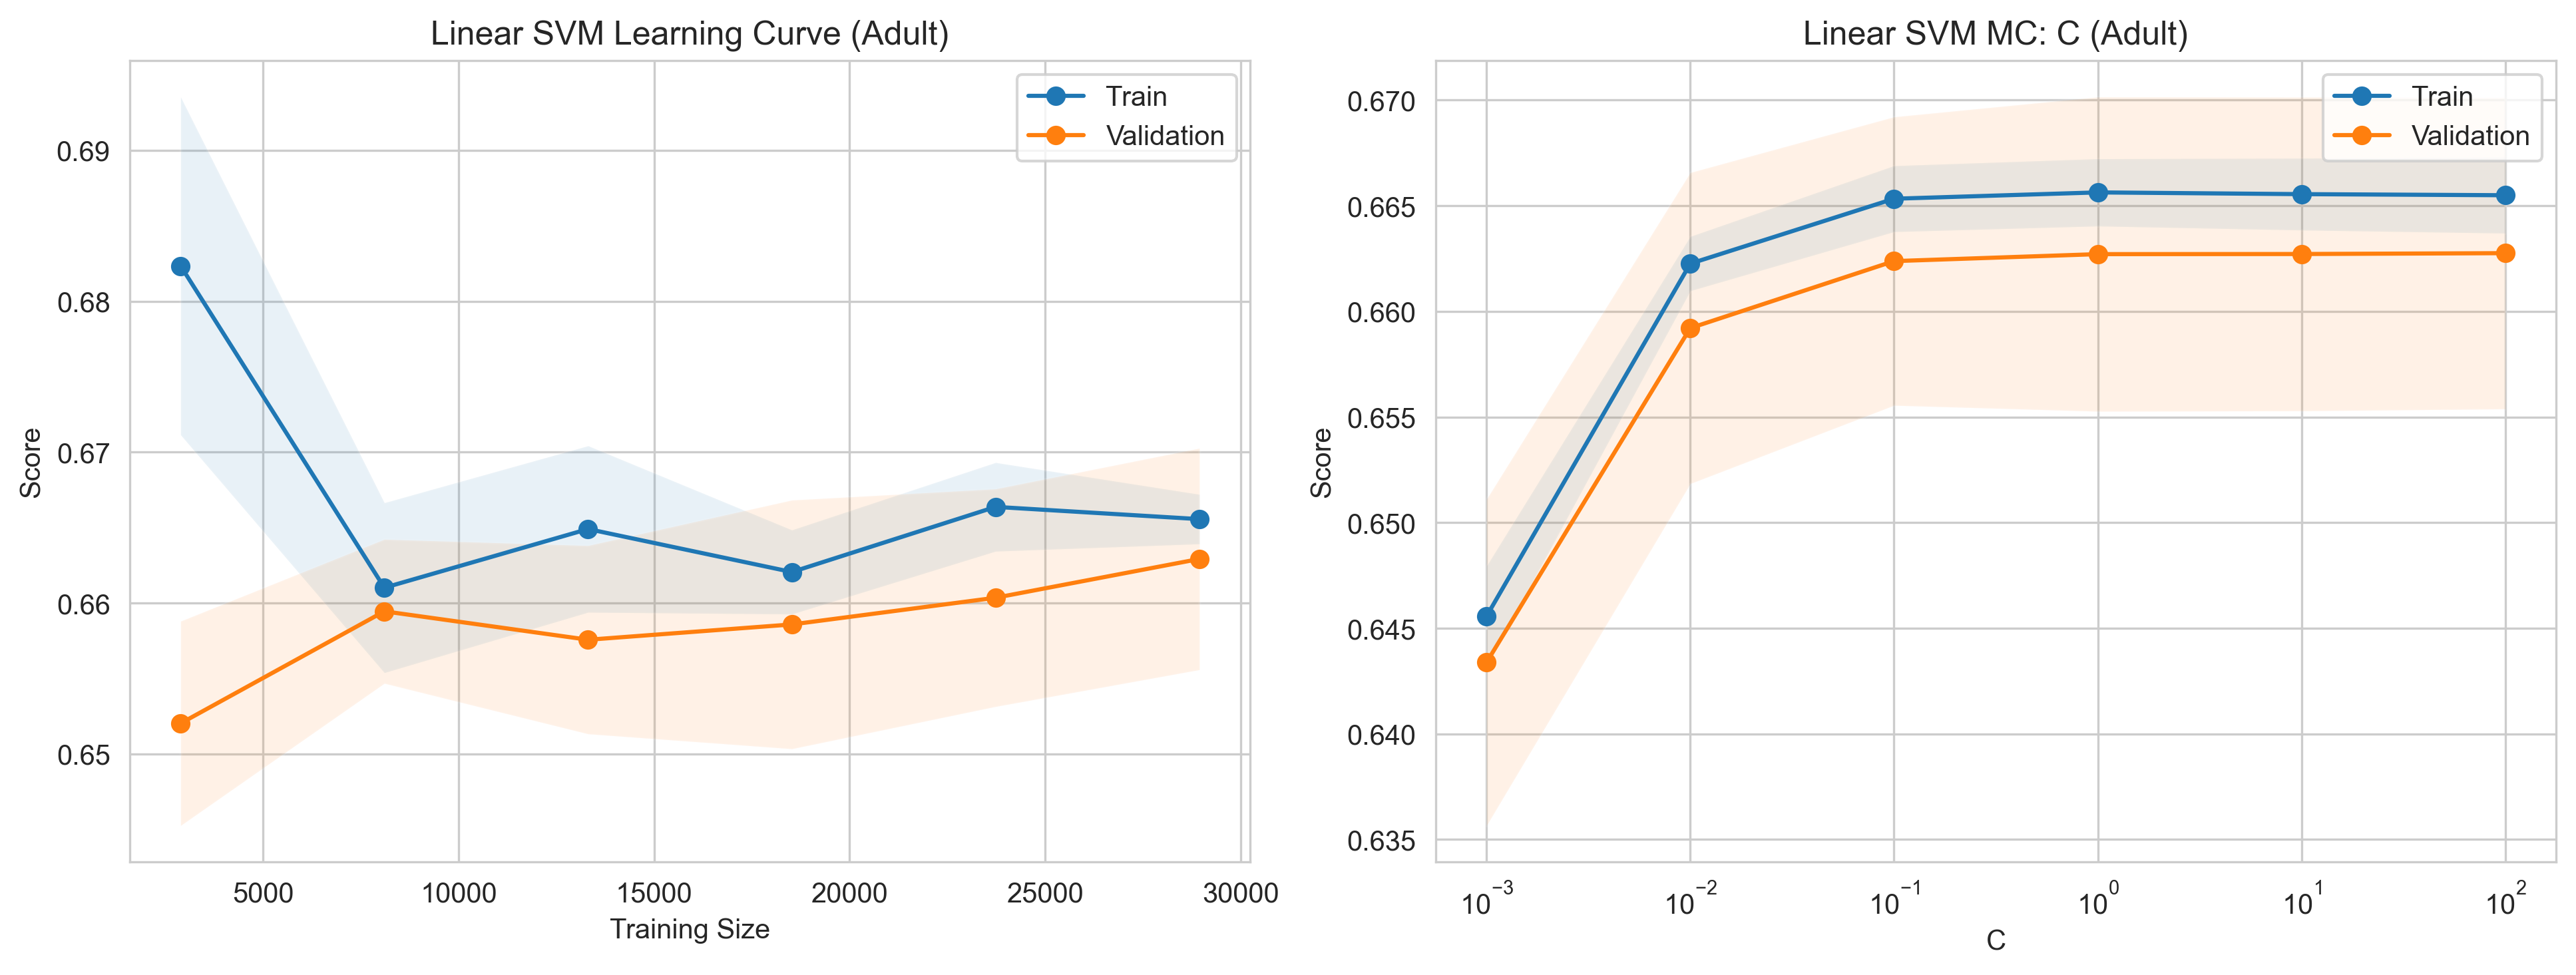
\includegraphics[width=\linewidth]{figures/svm_lin_adult_curves.png}
\caption{Linear SVM learning curve and model-complexity curve vs.\ $C$ (Adult). Validation F1 saturates near $C=1$, confirming approximate linear separability in the encoded feature space.}
\label{fig:svm_adult}
\end{figure}

\begin{figure}[H]
\centering
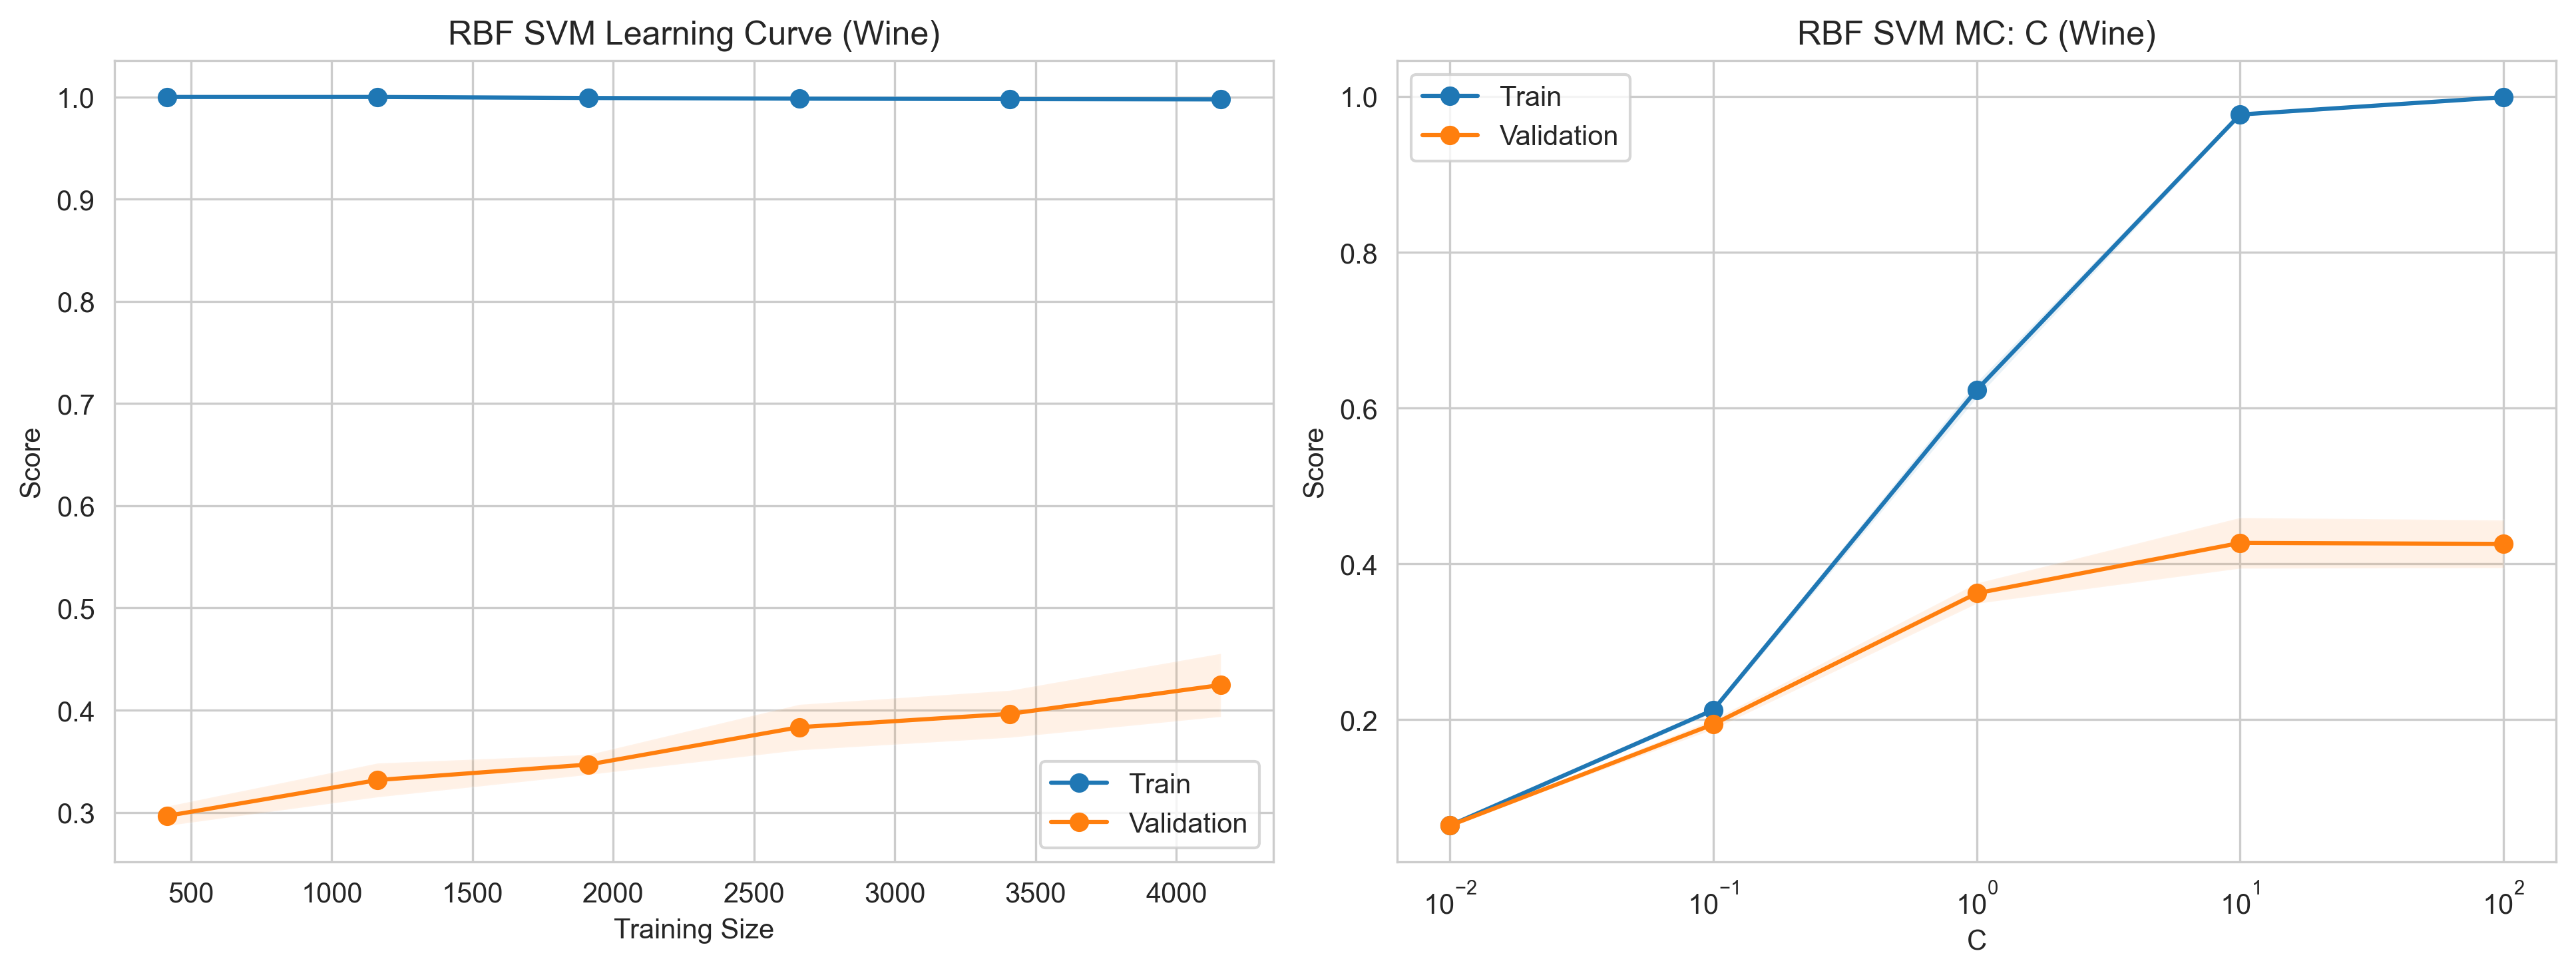
\includegraphics[width=\linewidth]{figures/svm_wine_curves.png}
\caption{RBF SVM learning and model-complexity curves (Wine). The large kernel gap (Linear F1$=$0.25 vs.\ RBF F1$=$0.47) demonstrates the importance of non-linear boundaries for this task.}
\label{fig:svm_wine}
\end{figure}

% ============================================================
\section{Neural Networks (scikit-learn)}
% ============================================================

We train \texttt{MLPClassifier} with \texttt{solver='sgd'} (no momentum, no Nesterov, no adaptive optimizers), tuning the number of hidden layers, layer width, L2 regularization ($\alpha$), learning rate, and batch size via Optuna. Early stopping with a 15\% validation fraction prevents overfitting.

\textbf{Adult.} The best architecture is a single hidden layer of 157 neurons ($\alpha=4 \times 10^{-4}$, $\text{lr}=0.052$, batch size$=$128), achieving accuracy$=$0.850 and F1$=$0.681, the highest F1 among all models on Adult. The epoch-based learning curve shows training loss steadily decreasing with validation score plateauing around epoch 50, indicating that early stopping is effectively preventing overfitting. The model-complexity curve against layer width shows validation F1 improving up to width$\approx$128, then flattening, suggesting that a single wide layer captures sufficient representational capacity for this task. The fit time of 125.4s reflects the SGD-only constraint: without momentum, convergence requires many more epochs with noisy gradients.

\textbf{Wine.} The best architecture uses three hidden layers of 63 neurons ($\alpha=3.2 \times 10^{-3}$, $\text{lr}=0.043$, batch size$=$64), but achieves only accuracy$=$0.535 and Macro-F1$=$0.285. The epoch curve reveals severe overfitting: training loss drops to near zero while validation performance stagnates. The SGD-only constraint is particularly damaging here: with only 5{,}197 training samples split across eight classes, each mini-batch provides a noisy, unrepresentative gradient signal. Without momentum or adaptive learning rates to smooth these updates, the optimizer bounces erratically and converges to sharp minima that memorize training patterns without generalizing.

\begin{figure}[H]
\centering
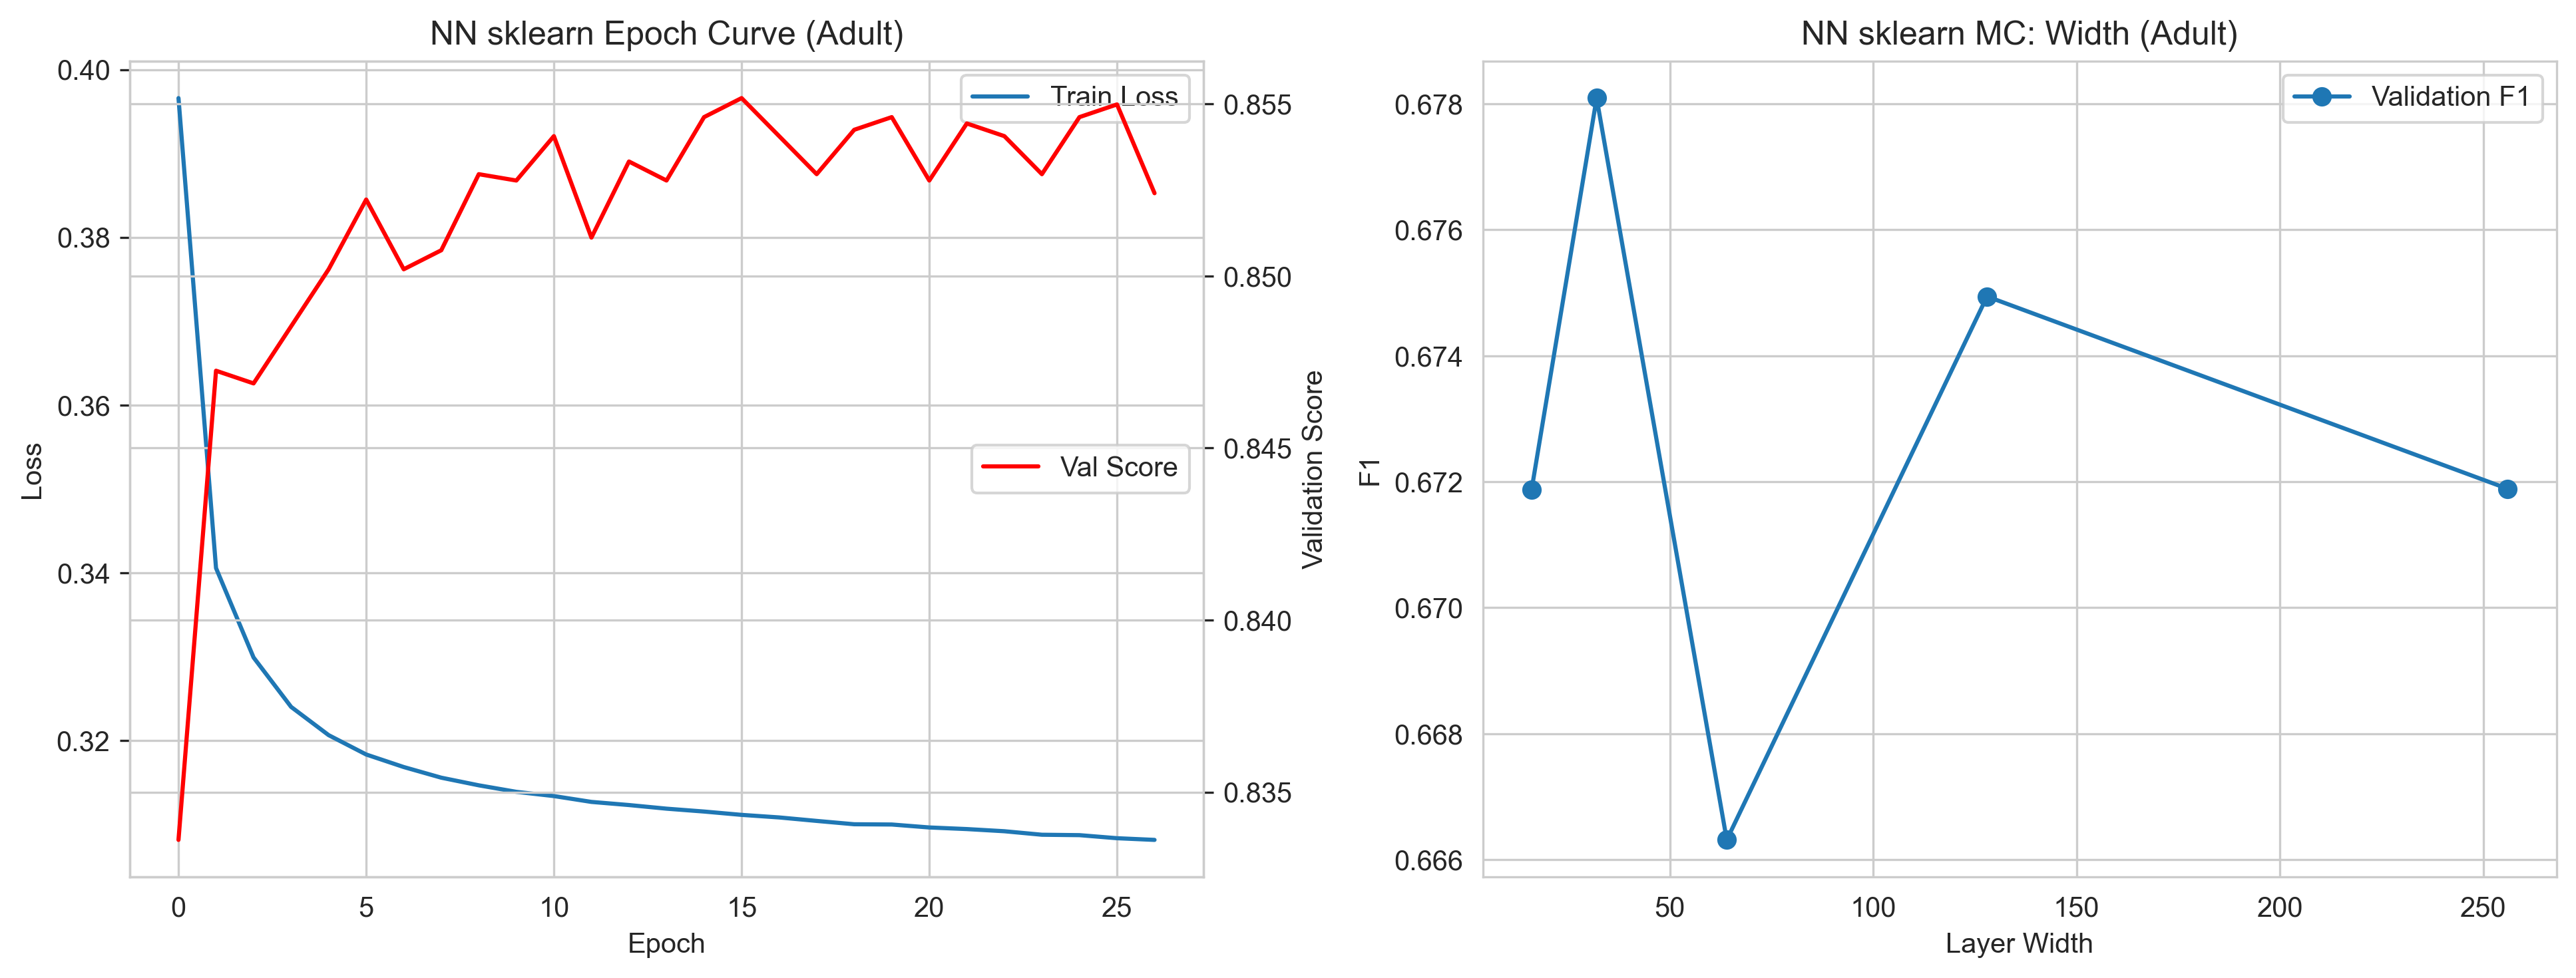
\includegraphics[width=\linewidth]{figures/nn_sklearn_adult_curves.png}
\caption{NN sklearn epoch curve and model-complexity curve vs.\ width (Adult). A single hidden layer of $\sim$128--157 neurons suffices; wider layers provide no additional benefit.}
\label{fig:nn_sk_adult}
\end{figure}

\begin{figure}[H]
\centering
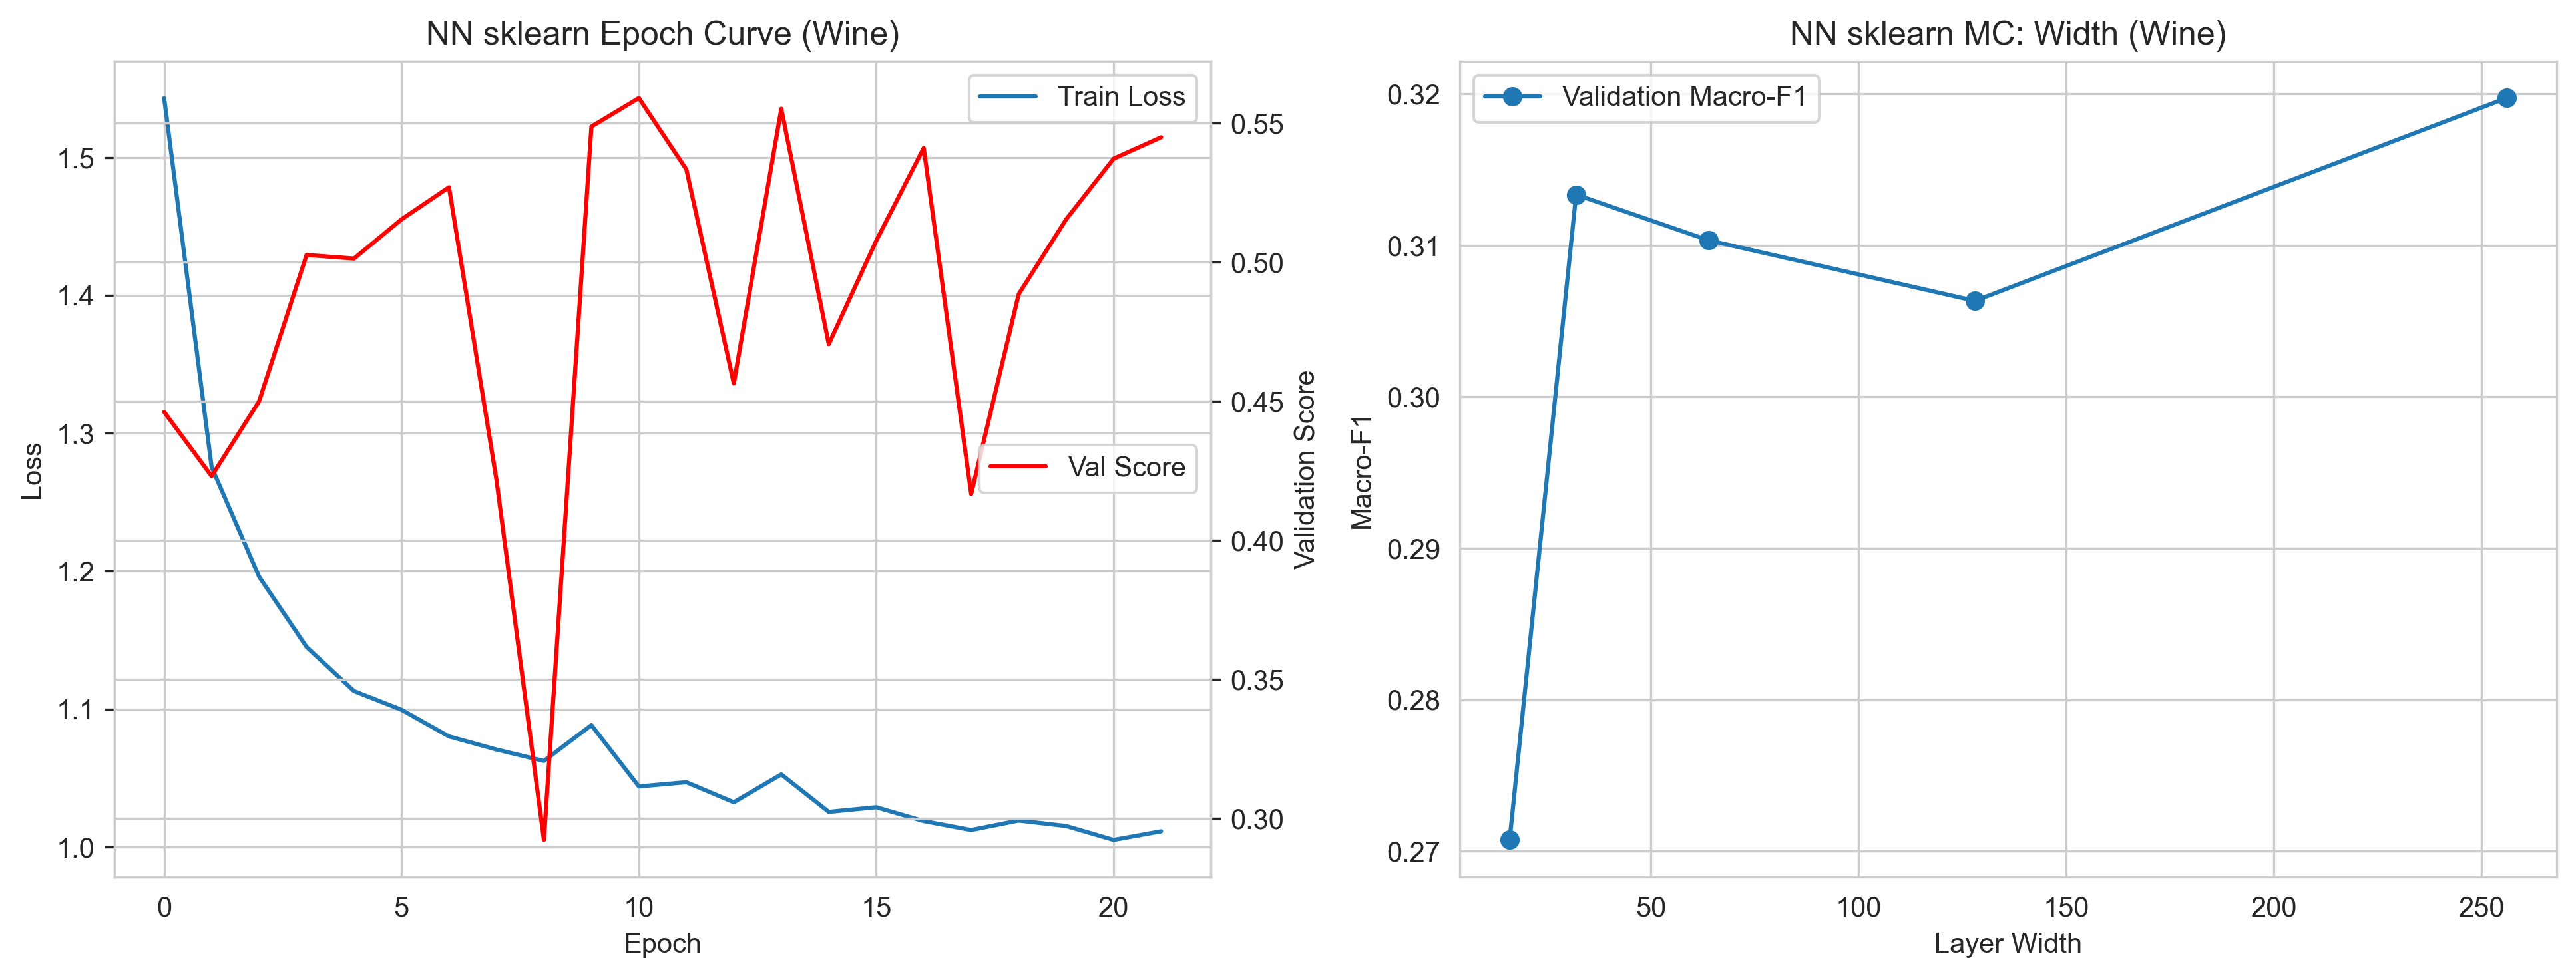
\includegraphics[width=\linewidth]{figures/nn_sklearn_wine_curves.png}
\caption{NN sklearn epoch curve and model-complexity curve (Wine). The divergence between training loss and validation score indicates severe overfitting under SGD-only constraints.}
\label{fig:nn_sk_wine}
\end{figure}

% ============================================================
\section{Neural Networks: PyTorch}
% ============================================================

We implement a custom \texttt{PytorchMLP} with configurable depth, width, activation function, and dropout ($p=0.2$), trained with plain SGD (no momentum). We compare two architectures per dataset: \textit{shallow-wide} and \textit{deep-narrow}, holding total parameter count approximately constant to isolate the effect of depth.

\textbf{Adult.} The shallow architecture (2 layers, $\sim$200 neurons each, 61{,}401 parameters) achieves validation F1$=$0.692 and test F1$=$0.673. The deep architecture (4 layers, $\sim$100 neurons each, 40{,}901 parameters) achieves validation F1$=$0.691 and test F1$=$0.691. Both train for 100 epochs in 31.1s and 21.4s respectively. The nearly identical performance suggests that depth provides no additional benefit on Adult when parameter count is held constant; the task is well-served by a single wide hidden layer, consistent with the sklearn result. The epoch curves show both architectures converging smoothly with train and validation F1 tracking closely, indicating healthy generalization under SGD.

\textbf{Wine.} The shallow architecture (2$\times$128, 19{,}208 parameters) achieves validation Macro-F1$=$0.316 and test Macro-F1$=$0.309. The deep architecture (4$\times$64, 13{,}832 parameters) performs worse with validation Macro-F1$=$0.269. The epoch curves show severe overfitting for both architectures, with training loss approaching zero while validation loss increases, the same pattern observed with sklearn. The deeper model degrades faster, likely because the vanishing gradient problem under plain SGD makes it harder to train deeper networks without momentum or residual connections.

\begin{figure}[H]
\centering
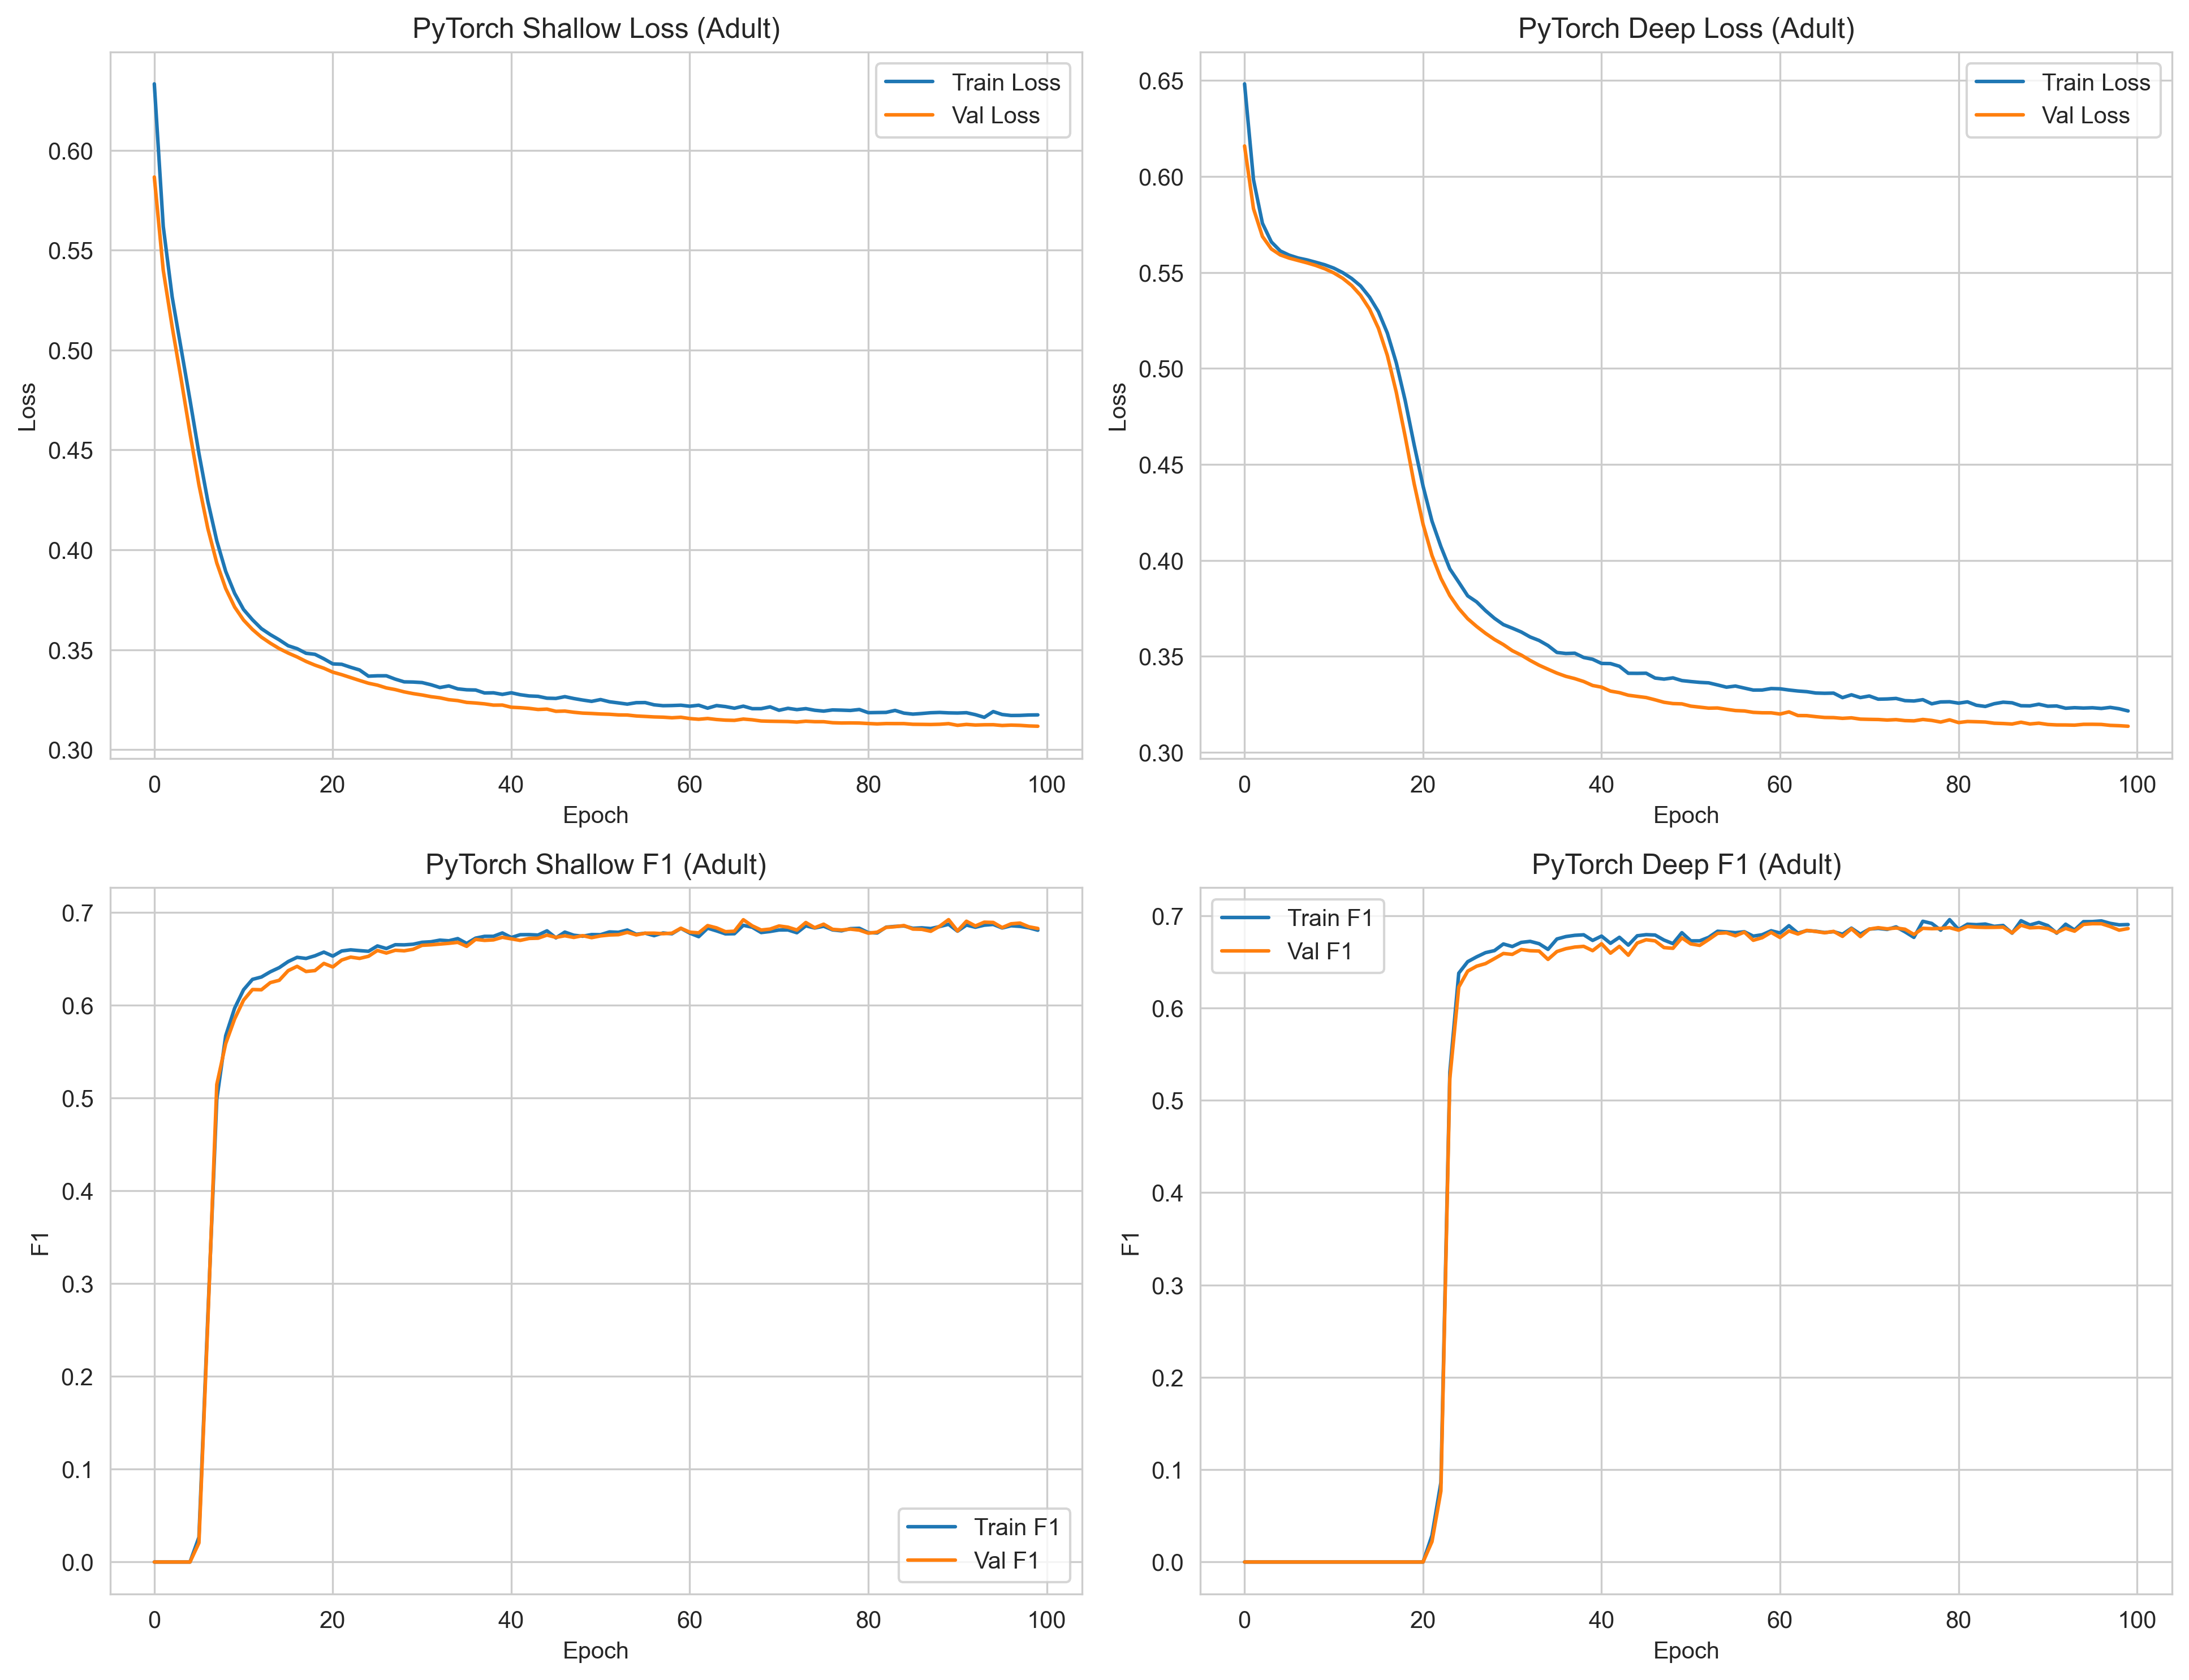
\includegraphics[width=\linewidth]{figures/nn_pytorch_adult_epochs.png}
\caption{PyTorch NN epoch curves for shallow and deep architectures (Adult). Both architectures converge similarly, indicating depth adds no benefit at constant parameter count for this task.}
\label{fig:nn_pt_adult}
\end{figure}

\begin{figure}[H]
\centering
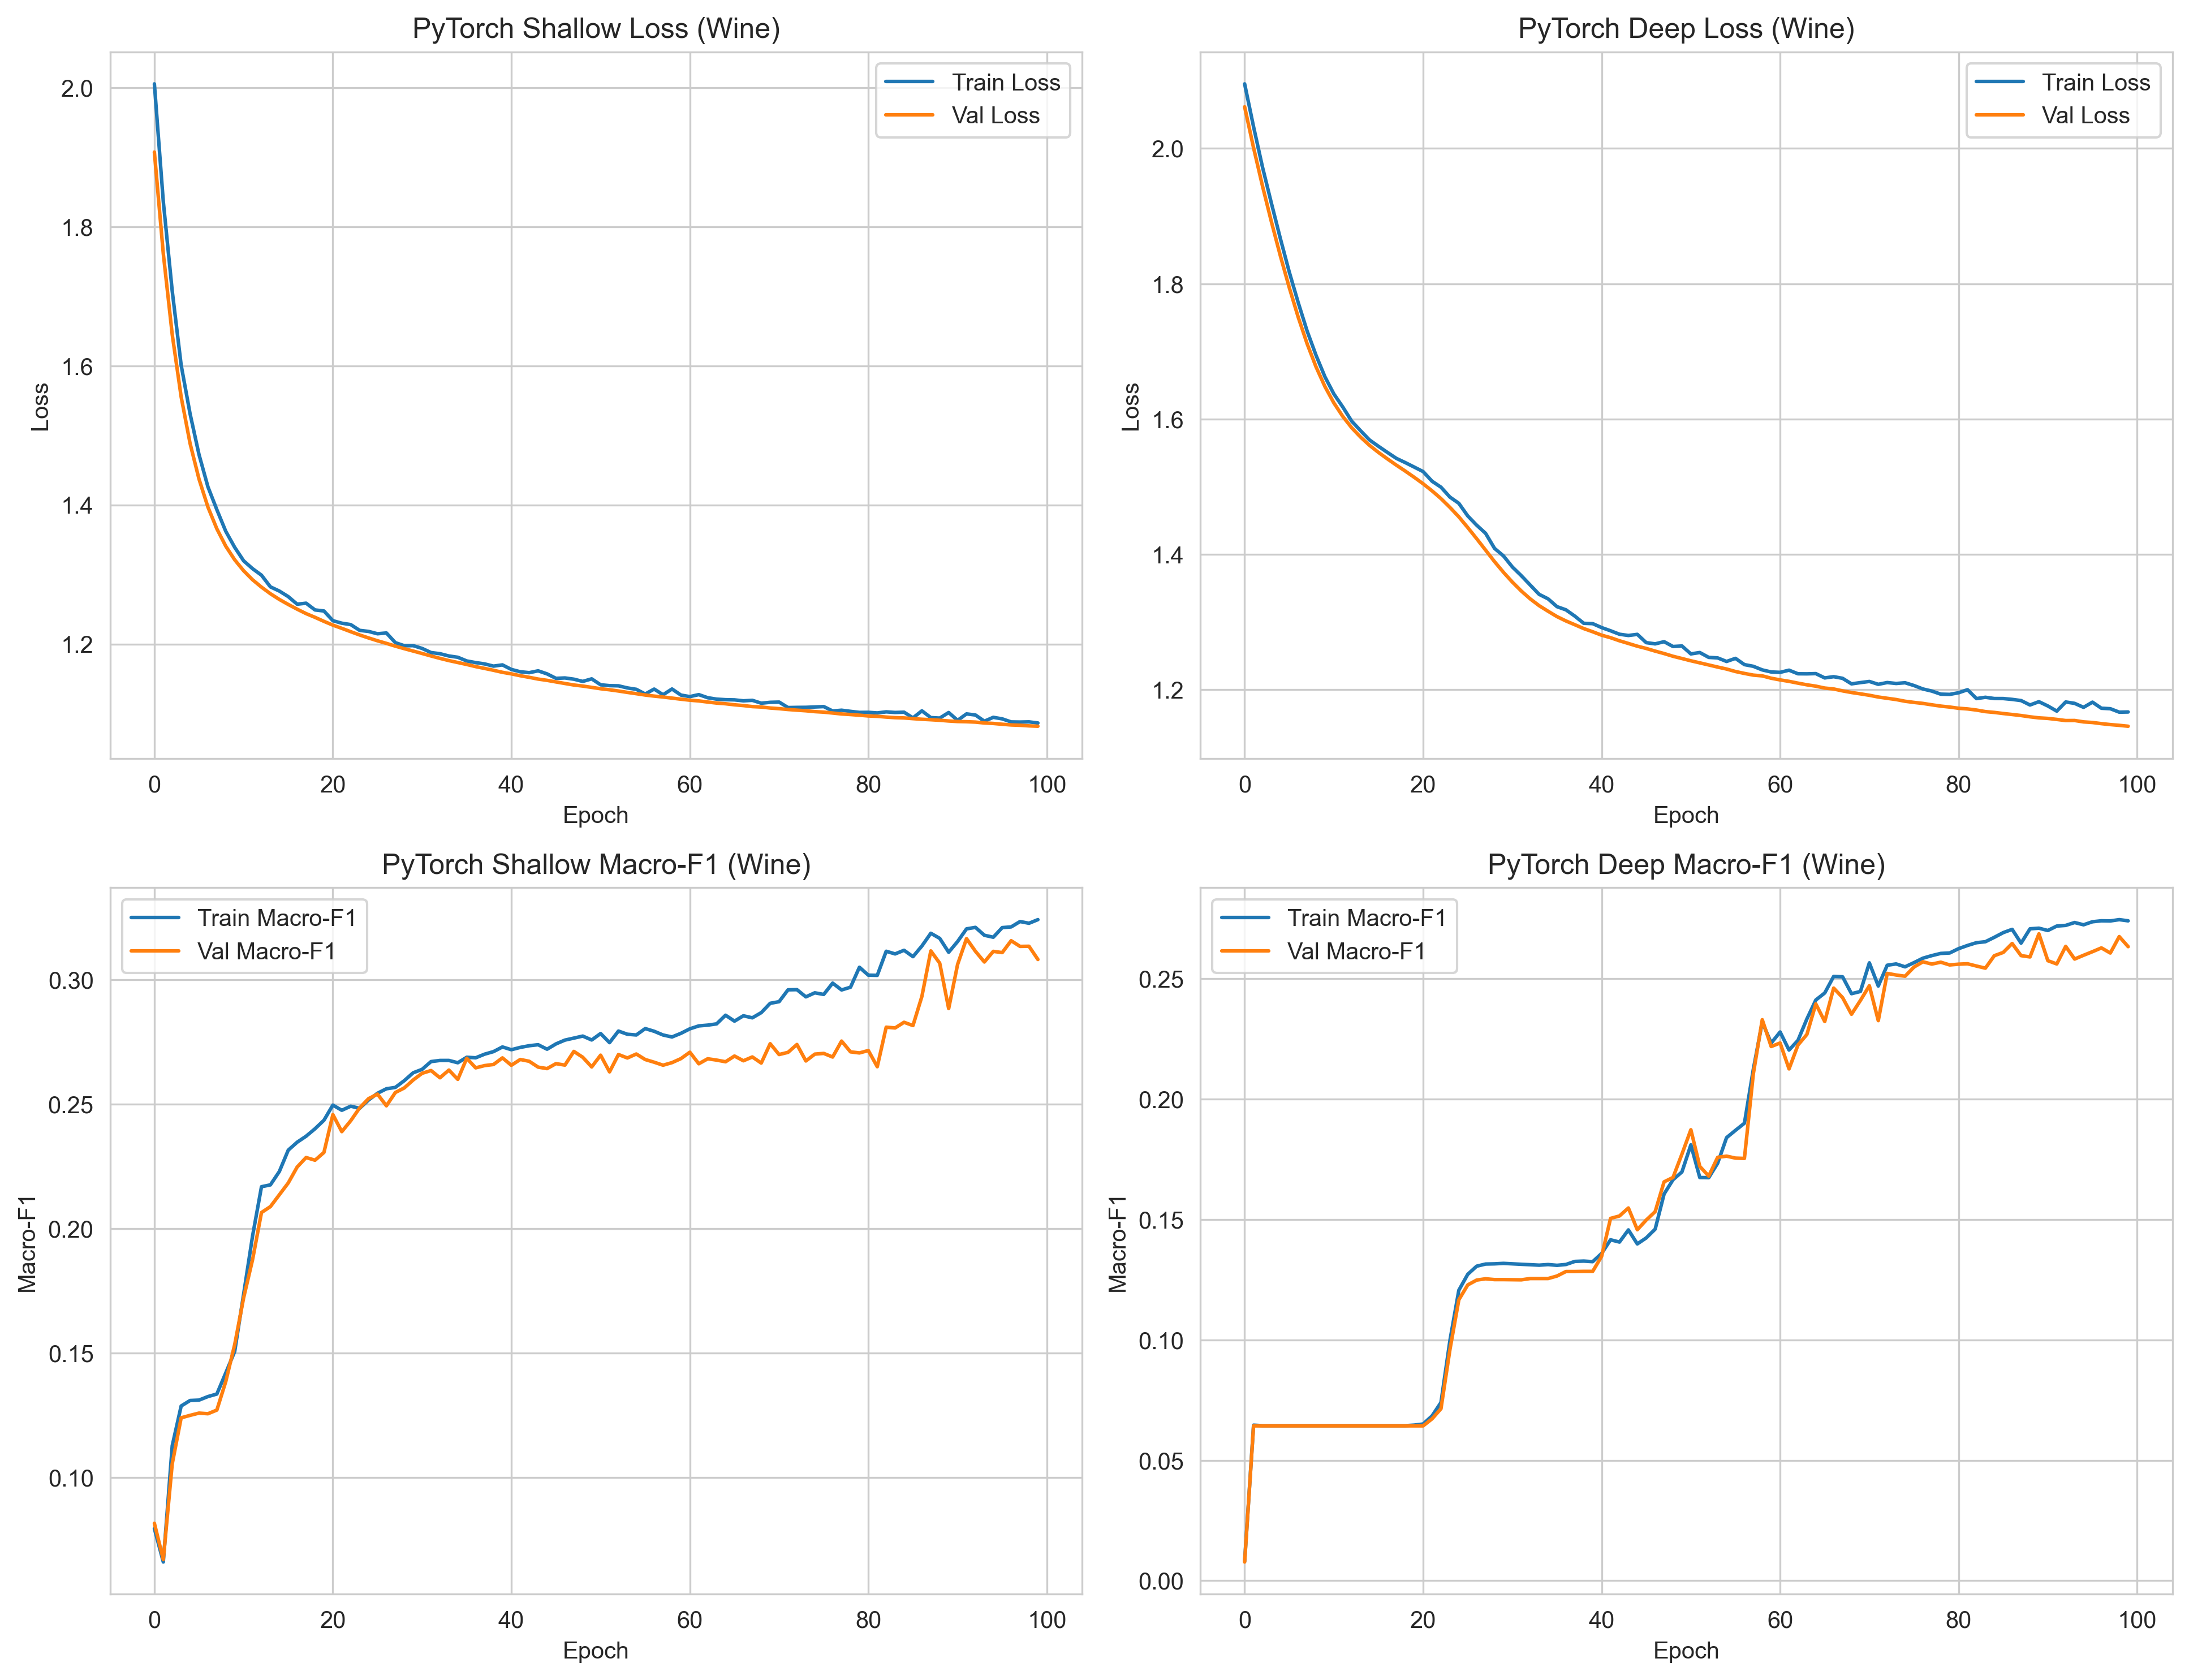
\includegraphics[width=\linewidth]{figures/nn_pytorch_wine_epochs.png}
\caption{PyTorch NN epoch curves (Wine). Both architectures overfit rapidly under SGD; the deeper model degrades further due to vanishing gradients without momentum.}
\label{fig:nn_pt_wine}
\end{figure}

% ============================================================
\section{Neural Network Comparison: scikit-learn vs.\ PyTorch}
% ============================================================

\begin{table}[H]
\centering
\caption{NN comparison under SGD-only constraints.}
\label{tab:nn_compare}
\small
\begin{tabular}{lcccc}
\toprule
& \multicolumn{2}{c}{\textbf{Adult}} & \multicolumn{2}{c}{\textbf{Wine}} \\
\cmidrule(lr){2-3} \cmidrule(lr){4-5}
Metric & sklearn & PyTorch & sklearn & PyTorch \\
\midrule
Accuracy & 0.850 & 0.851 & 0.535 & 0.564 \\
F1 / Macro-F1 & 0.681 & 0.673 & 0.285 & 0.309 \\
Fit time (s) & 125.4 & 31.1 & 1.7 & 2.7 \\
Predict time (s) & 0.016 & 0.005 & 0.039 & 0.002 \\
\bottomrule
\end{tabular}
\end{table}

Both implementations achieve comparable accuracy and F1 under the same SGD constraint, confirming that the poor Wine results are an optimizer limitation, not an implementation artifact. The key differences lie in runtime and flexibility. On the large Adult dataset, PyTorch is 4$\times$ faster (31s vs.\ 125s), likely due to differences in batching strategy and internal convergence behavior rather than language-level overhead, as both frameworks use optimized compiled backends. On the small Wine dataset, the relationship inverts: sklearn (1.7s) is faster than PyTorch (2.7s) because the matrix operations are trivially fast for both, and sklearn's single \texttt{.fit()} call avoids the per-epoch bookkeeping of PyTorch's explicit training loop.

From a tunability perspective, PyTorch offers full control over architecture, training schedule, and epoch-level behavior, enabling the shallow-vs-deep comparison. Sklearn provides a more constrained but simpler interface that is sufficient for standard MLP experiments. Under the SGD-only constraint, neither framework can overcome the fundamental challenge of training on small, imbalanced data without adaptive optimizers.

% ============================================================
\section{Cross-Model Comparison}
% ============================================================

\begin{table}[H]
\centering
\caption{Cross-model comparison (Adult).}
\label{tab:adult_compare}
\small
\begin{tabular}{lcccc}
\toprule
Model & Accuracy & F1 & Fit (s) & Predict (s) \\
\midrule
DT       & 0.854 & 0.670 & 0.162 & 0.001 \\
kNN      & 0.836 & 0.642 & 0.001 & 0.796 \\
SVM-Lin  & 0.846 & 0.654 & 0.114 & 0.000 \\
SVM-RBF  & 0.848 & 0.650 & 1.353 & 2.393 \\
NN-sklearn & 0.850 & 0.681 & 125.4 & 0.016 \\
NN-PyTorch & 0.851 & 0.673 & 31.1  & 0.005 \\
\bottomrule
\end{tabular}
\end{table}

\begin{table}[H]
\centering
\caption{Cross-model comparison (Wine).}
\label{tab:wine_compare}
\small
\begin{tabular}{lcccc}
\toprule
Model & Accuracy & Macro-F1 & Fit (s) & Predict (s) \\
\midrule
DT       & 0.609 & 0.432 & 0.021 & 0.000 \\
kNN      & 0.679 & 0.455 & 0.001 & 0.043 \\
SVM-Lin  & 0.518 & 0.253 & 0.027 & 0.000 \\
SVM-RBF  & 0.662 & 0.467 & 0.480 & 0.145 \\
NN-sklearn & 0.535 & 0.285 & 1.730 & 0.039 \\
NN-PyTorch & 0.564 & 0.309 & 2.683 & 0.002 \\
\bottomrule
\end{tabular}
\end{table}

On Adult, all models cluster within a narrow F1 range (0.642--0.681), with NNs edging ahead and kNN trailing. The tight spread suggests that Adult is a well-structured problem where even simple algorithms extract most of the learnable signal. The practical takeaway is that DT offers the best efficiency tradeoff: it achieves F1$=$0.670 (within 0.01 of the best NN) with 0.163s total compute, compared to the NN's 125--156s.

On Wine, the picture reverses dramatically. SVM-RBF leads (Macro-F1$=$0.467), followed closely by kNN (0.455) and DT (0.432), while both NNs collapse to 0.285--0.309. This contradicts the hypothesis that NNs would dominate and confirms the no-free-lunch theorem: algorithm performance is dataset-dependent. The NNs' failure stems from the SGD-only constraint on a small (5{,}197 samples), highly imbalanced (8 classes) dataset. Plain SGD produces noisy gradients that drive the model into sharp, non-generalizing minima. Simpler models with fewer parameters and stronger inductive biases (kNN's locality assumption, SVM's margin maximization, DT's axis-aligned partitioning) prove more robust in this low-data regime.

The cross-dataset comparison reveals a bias--variance spectrum. DT and kNN are high-variance, low-bias learners that adapt well to data structure but risk overfitting. SVM-RBF balances flexibility with margin-based regularization, making it the most consistent performer across both datasets. NNs have the highest capacity but require sufficient data and effective optimization to realize it.

\begin{figure}[H]
\centering
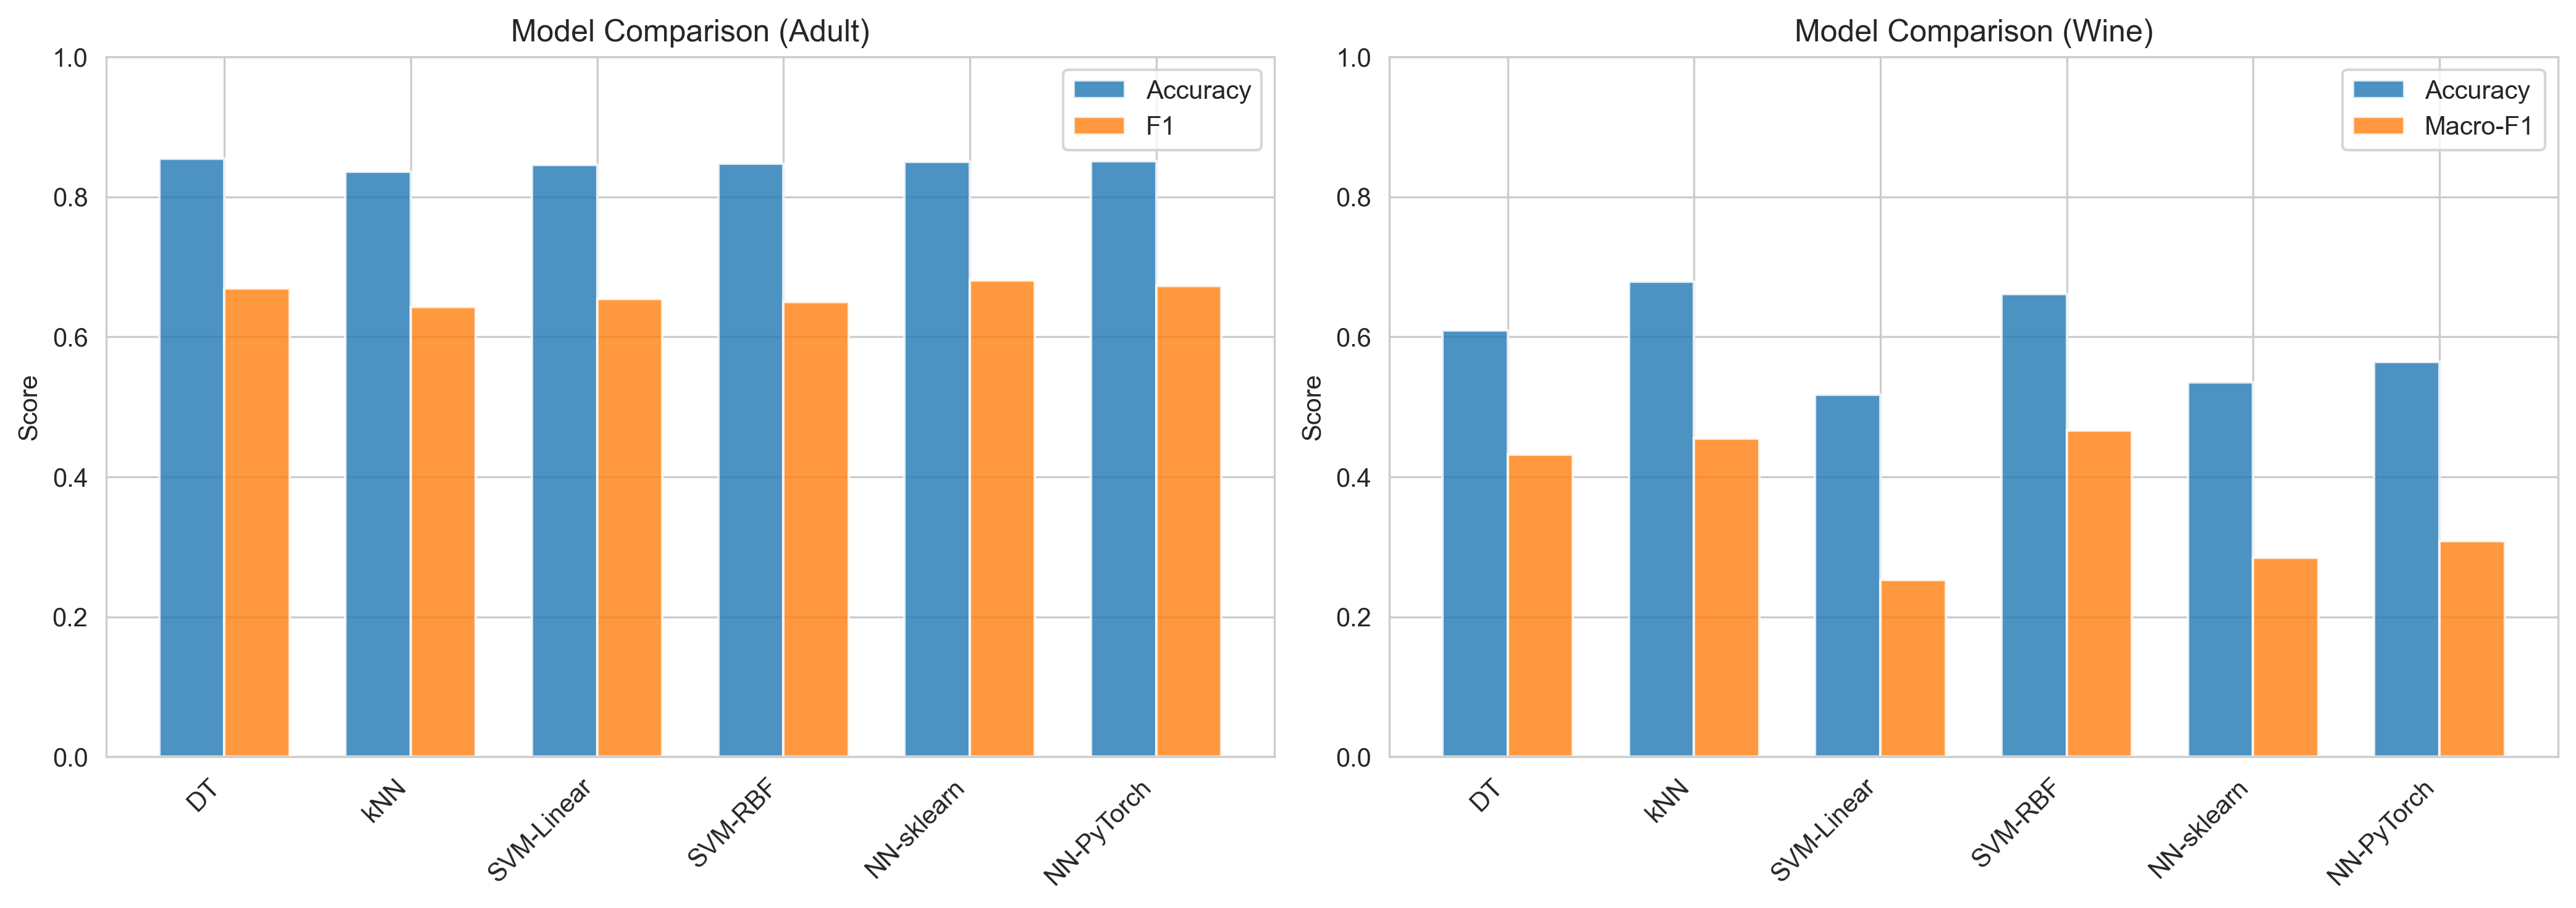
\includegraphics[width=\linewidth]{figures/cross_model_comparison.png}
\caption{Cross-model accuracy and F1/Macro-F1 comparison. Adult shows tight clustering with NN slightly ahead; Wine shows substantial divergence with SVM-RBF and kNN leading.}
\label{fig:cross_model}
\end{figure}

% ============================================================
\section{Leakage / Evaluation Debug}
\label{sec:leakage}
% ============================================================

To verify that our results reflect genuine learning rather than data leakage, we run two diagnostic baselines on both datasets.

The \textbf{dummy baseline} (most-frequent class) achieves accuracy$=$0.752 and F1$=$0.000 on Adult, and accuracy$=$0.346 and Macro-F1$=$0.064 on Wine. The zero F1 on Adult confirms that the 75\% accuracy of a naive classifier is entirely driven by class imbalance, not learning. All trained models substantially exceed both dummy metrics.

The \textbf{shuffled-label baseline} trains a DT (\texttt{max\_depth}$=$10) on randomly permuted training labels. This achieves F1$=$0.034 on Adult and Macro-F1$=$0.113 on Wine, near-chance performance, as expected when the feature--target relationship is destroyed. Our best models (NN-sklearn F1$=$0.681 on Adult, SVM-RBF Macro-F1$=$0.467 on Wine) achieve 20$\times$ and 4$\times$ higher scores respectively, confirming no leakage in the evaluation pipeline.

% ============================================================
\section{Extra Credit: Activation Function Study}
% ============================================================

Using the Adult dataset and the deep PyTorch architecture (4$\times$100, SGD only), we compare four activation functions (ReLU, GELU, SiLU/Swish, and Tanh) holding architecture, preprocessing, regularization, and training protocol constant.

\begin{table}[H]
\centering
\caption{Activation function comparison (Adult, SGD only).}
\label{tab:activation}
\small
\begin{tabular}{lcccc}
\toprule
Activation & Test Acc & Test F1 & Best Val F1 & Epochs \\
\midrule
ReLU & 0.851 & 0.682 & 0.690 & 100 \\
Tanh & 0.846 & 0.656 & 0.675 & 100 \\
GELU & 0.836 & 0.627 & 0.625 & 100 \\
SiLU & 0.829 & 0.599 & 0.614 & 100 \\
\bottomrule
\end{tabular}
\end{table}

ReLU outperforms all alternatives under SGD-only training. Its piecewise-linear gradient (exactly 0 or 1) provides the cleanest gradient signal, which is critical when the optimizer has no momentum to smooth noisy updates. Tanh ranks second, likely because its zero-centered outputs help gradient flow compared to sigmoid-like activations, though its saturating tails ($\tanh(x) \to \pm 1$) slow convergence for large activations. GELU and SiLU, which are smooth approximations of ReLU designed to work well with adaptive optimizers like Adam, perform worst under SGD. Their smoother gradients introduce additional curvature that adaptive optimizers can exploit but plain SGD cannot, resulting in slower convergence and lower final performance. All four activations train for the full 100 epochs without triggering early stopping, suggesting that SGD's slow convergence rate is the binding constraint regardless of activation choice.

\begin{figure}[H]
\centering
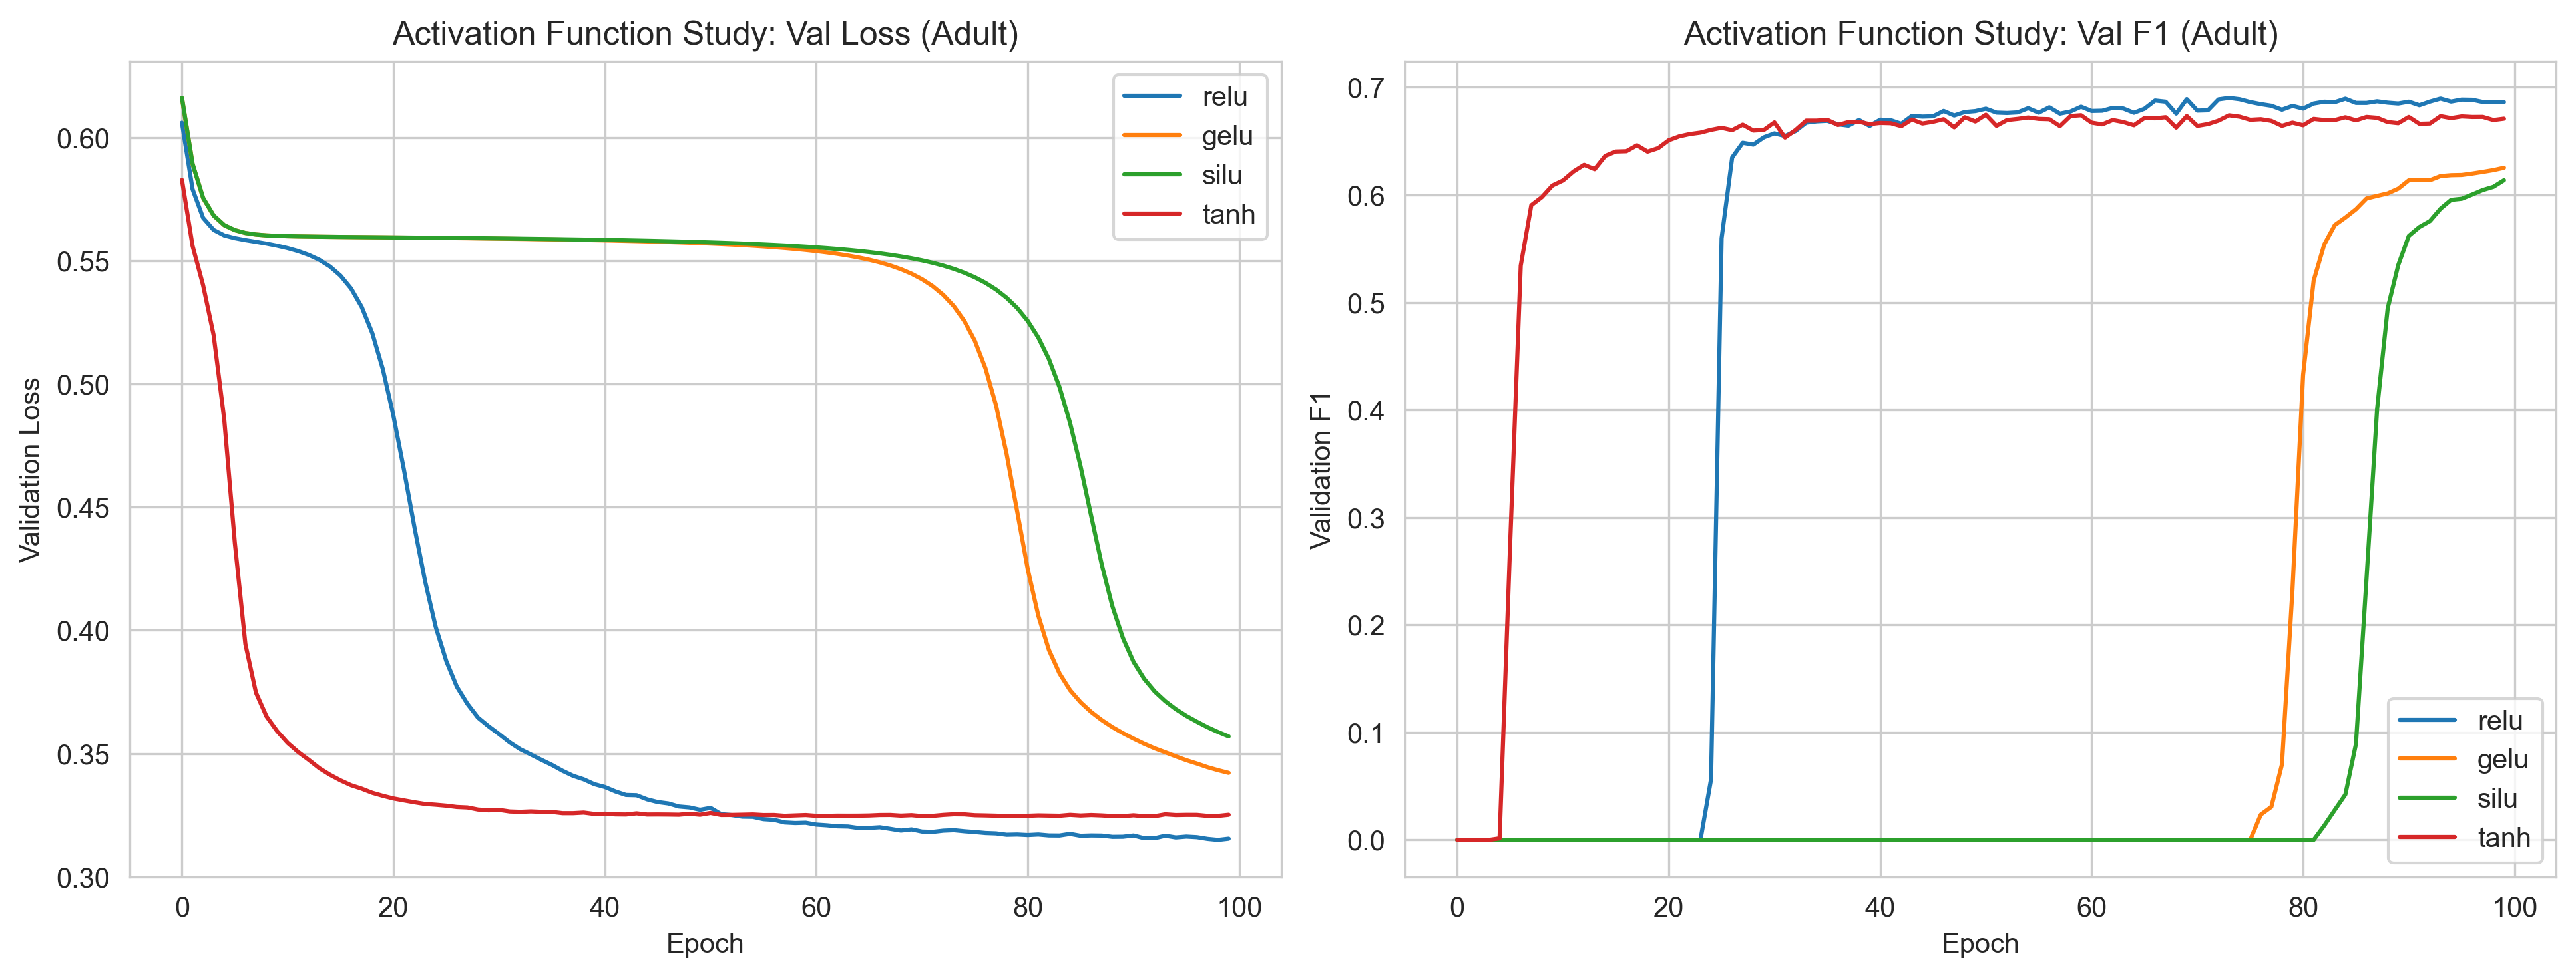
\includegraphics[width=\linewidth]{figures/extra_credit_activations.png}
\caption{Activation function study: validation loss and F1 across epochs (Adult). ReLU converges fastest and reaches the highest F1 under SGD-only training.}
\label{fig:activations}
\end{figure}

% ============================================================
\section{Conclusion}
% ============================================================

Our results partially support and partially contradict the initial hypotheses, providing several insights into supervised learning behavior across distinct dataset regimes.

On Adult, the predicted ordering (SVM $\geq$ NN $>$ DT $>$ kNN) was partially confirmed: NNs achieved the highest F1, and kNN finished last. However, DT (F1$=$0.670) outperformed both SVM variants (F1$\leq$0.654), likely because the axis-aligned splits align well with the sparse binary features created by one-hot encoding. On Wine, the predicted ordering (NN $\geq$ DT $>$ kNN $>$ SVM) was substantially contradicted: NNs collapsed to last place while SVM-RBF and kNN led. This reversal demonstrates that algorithm performance is fundamentally dataset-dependent, consistent with the no-free-lunch theorem~\cite{wolpert1997no}.

Regarding Type~I and Type~II errors, the Adult confusion matrices reveal that all models exhibit higher false-negative rates (predicting $\leq$50K for individuals earning $>$50K) than false-positive rates, reflecting the 3:1 class prior. In a deployment context, this asymmetry has policy implications: a model used for targeted benefits would systematically exclude eligible high-income individuals. For Wine, the multi-class confusion matrices show that errors concentrate between adjacent quality levels (e.g., predicting quality 4 as 3 or 5), which is unsurprising given the ordinal nature of the target and the subjective basis of human quality ratings.

As a realistic next step, we would apply class-rebalancing techniques (SMOTE, class-weight adjustments) to improve minority-class performance, particularly for Wine where rare quality ratings (1, 2, 7, 8) constitute only 6.2\% of samples. Additionally, removing the SGD-only constraint and using Adam with learning-rate scheduling would likely improve NN performance substantially on Wine, isolating how much of the poor performance is attributable to the optimizer versus the data.

\paragraph{AI Use Statement.} I used GitHub Copilot CLI to assist with code generation, debugging, and outlining sections of this report. I reviewed, verified, and understand all assisted content.

\bibliographystyle{ieeetr}
\begin{thebibliography}{2}
\bibitem{hastie2009elements}
T.~Hastie, R.~Tibshirani, and J.~Friedman, \textit{The Elements of Statistical Learning: Data Mining, Inference, and Prediction}, 2nd~ed. New York: Springer, 2009.

\bibitem{wolpert1997no}
D.~H.~Wolpert and W.~G.~Macready, ``No free lunch theorems for optimization,'' \textit{IEEE Transactions on Evolutionary Computation}, vol.~1, no.~1, pp.~67--82, 1997.
\end{thebibliography}

\end{document}
